\documentclass[11pt,a4paper]{article}

% =================================================================
% PAQUETES Y CONFIGURACIÓN GENERAL
% =================================================================
\usepackage[utf8]{inputenc}
\usepackage[T1]{fontenc}
\usepackage[spanish,es-tabla]{babel}
\usepackage{amsmath,amssymb}
\usepackage{array}
\usepackage{graphicx}
\usepackage{geometry}
\geometry{a4paper, margin=2.5cm}
\usepackage[nopatch=footnote]{microtype}
\usepackage{booktabs}
\usepackage{float}
\usepackage{caption}
\usepackage{subcaption}
\usepackage{xcolor}
\usepackage{titlesec}
\usepackage{fancyhdr}
\usepackage[titles]{tocloft}
\usepackage[colorlinks=true,linkcolor=blue,urlcolor=blue,citecolor=blue,hypertexnames=false]{hyperref}
\usepackage{bookmark}
\usepackage{xurl}

\hypersetup{
    pdftitle={Estudio de las comunicaciones en un entorno IoT},
    pdfauthor={Grupo\_03},
    bookmarksnumbered=true,
    bookmarksopen=true
}
\bookmarksetup{numbered}

% Puntos conductores en el índice
\renewcommand{\cftsecleader}{\cftdotfill{\cftdotsep}}
\renewcommand{\cftsubsecleader}{\cftdotfill{\cftdotsep}}
\renewcommand{\cftsecfont}{\small\bfseries}
\renewcommand{\cftsecpagefont}{\small\bfseries}
\renewcommand{\cftsubsecfont}{\small}
\renewcommand{\cftsubsecpagefont}{\small}
\setlength{\cftbeforesecskip}{2pt}
\setlength{\cftbeforesubsecskip}{0pt}

% Columnas de tabla alineadas a la izquierda
\newcolumntype{L}[1]{>{\raggedright\arraybackslash}p{#1}}

% Colores corporativos
\definecolor{upvred}{RGB}{180, 0, 40}
\definecolor{darkblue}{RGB}{0, 40, 100}

% Estilo de títulos
\titleformat{\section}
  {\normalfont\Large\bfseries\color{darkblue}}{\thesection}{1em}{}
\titleformat{\subsection}
  {\normalfont\large\bfseries\color{darkblue}}{\thesubsection}{1em}{}

% Encabezado y pie de página
\pagestyle{fancy}
\fancyhf{}
\lhead{\small \textbf{MUCC -- SCO}}
\rhead{\small \textbf{Seguimiento logístico de paquetes}}
\lfoot{\small Grupo\_03}
\rfoot{\small Página \thepage}
\renewcommand{\headrulewidth}{0.4pt}
\renewcommand{\footrulewidth}{0.4pt}

% Figuras y tablas
\captionsetup{font=small,labelfont=bf,justification=centering}
\setlength{\emergencystretch}{2em}

\addto\captionsspanish{\renewcommand{\contentsname}{Tabla de contenidos}}

% =================================================================
% DATOS EDITABLES DEL TRABAJO
% =================================================================
\newcommand{\tituloTrabajo}{Estudio de las comunicaciones en un entorno IoT}
\newcommand{\asignatura}{Seguridad de las Cosas (SCO)}
\newcommand{\titulacion}{Máster Universitario en Ciberseguridad y Ciberinteligencia (MUCC)}
\newcommand{\profesor}{Mario Aragonés Lozano}
\newcommand{\fechaPortada}{1 de noviembre de 2026}
% Autores: sustituir los textos entre llaves por los nombres reales

\newcommand{\autorUno}{Lucía Alba Torres}
\newcommand{\autorDos}{Juan Pablo Bueno Fuentes}
\newcommand{\autorTres}{Luis Clemente Pascual}
\newcommand{\autorCuatro}{Juan Carlos González Arjona}
\newcommand{\autorCinco}{Álvaro García Sáez}


% ================================================================= 
% FORMATO DE PÁRRAFO E INTERLINEADO 
% ================================================================= 
% 1\. Interlineado a 1.5 líneas 
\usepackage{setspace} 
\onehalfspacing 

% 2\. Espaciado entre párrafos (0 pt antes, 6 pt después) 
\setlength{\parskip}{6pt}
% 3\. Sangría de primera línea 
\setlength{\parindent}{1cm} 

\begin{document} 

% ================================================================= 
% PORTADA INSTITUCIONAL 
% ================================================================= 
\begin{titlepage}
    \centering

    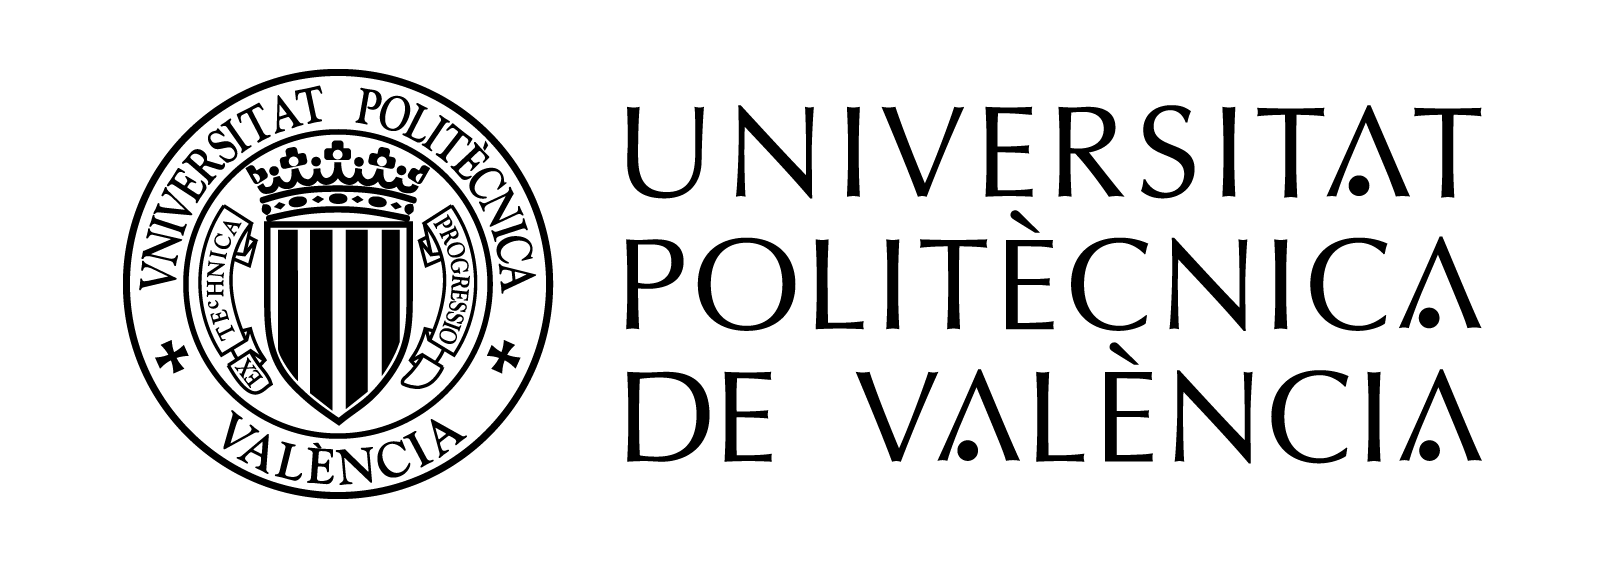
\includegraphics[height=2.5cm]{upv_logo.png}\par
    \vspace{0.8cm}

    {\Large \textbf{UNIVERSITAT POLITÈCNICA DE VALÈNCIA}}\\[0.3cm]
    {\large \textbf{Escola Tècnica Superior d'Enginyeria Informàtica}}\\[1.2cm]

    {\huge \textbf{\textcolor{upvred}{Seguridad de las Cosas (SCO)}}}\\[0.6cm]
    {\Large \textbf{\tituloTrabajo}}\\[0.5cm]
    {\large \titulacion}\\[1.0cm]

    \rule{\linewidth}{0.5mm}\\[0.8cm]

    \begin{center}
        \begin{tabular}{@{}L{0.45\textwidth} L{0.45\textwidth}@{}}
            \large \textbf{\autorUno}   & \large \textbf{\autorDos}   \\[0.35cm]
            \large \textbf{\autorTres}  & \large \textbf{\autorCuatro}\\[0.35cm]
            \large \textbf{\autorCinco} & 
        \end{tabular}
    \end{center}\vspace{0.8cm}

    \begin{minipage}{0.92\textwidth}
        \centering \small
        \begin{tabular}{@{}r@{\hspace{0.45cm}}L{0.73\textwidth}@{}}
            \textbf{Titulación:} & \titulacion \\[0.2cm]
            \textbf{Asignatura:} & \asignatura \\[0.2cm]
            \textbf{Profesor:}   & \profesor \\[0.2cm]
            \textbf{Fecha:}      & \fechaPortada \\
        \end{tabular}
    \end{minipage}

    \vfill
    
\includegraphics[height=1.6cm]{etsinf_logo.png}
\end{titlepage}

% =================================================================
% ÍNDICES INTERACTIVOS
% =================================================================
\tableofcontents
\newpage
\listoffigures
\newpage
\listoftables
\newpage

% =================================================================
% 1. INTRODUCCIÓN
% =================================================================
\clearpage
\section{Introducción}
\label{sec:apartado1}

Para las empresas de logística el seguimiento de sus paquetes durante su transporte es un aspecto fundamental, ya que permite conocer la ubicación de los mismos, controlar los tiempos de entrega y mejorar la eficiencia de los procesos de distribución. Para conseguirlo, es necesario disponer de un sistema capaz de registrar la posición de cada paquete a lo largo de todo su recorrido y transmitir esta información a una plataforma de gestión.

No obstante, desarrollar un sistema con estas características no es un reto trivial, puesto que las condiciones de localización y comunicación varían en función del entorno por el que se desplace la mercancía. Mientras que en carreteras y zonas abiertas suele ser posible utilizar sistemas de posicionamiento por satélite, en entornos urbanos y espacios interiores la precisión puede verse reducida. Además, en entornos subterráneos como los túneles, pueden no estar disponibles las comunicaciones convencionales, lo que hace necesario estudiar y planear soluciones adaptadas.

El objetivo principal de este trabajo es diseñar una pequeña propuesta de sistema de seguimiento de paquetes que nos permita conocer su ubicación y el tiempo transcurrido desde su recogida hasta su entrega al cliente. Para ello, vamos a estudiar características de los distintos escenarios que pueden darse, las tecnologías de localización disponibles, y los sensores que deberían incorporarse teniendo en cuenta las necesidades y restricciones.

En la Figura~\ref{fig:vision_general} se resume la arquitectura completa del sistema propuesto, desde la recogida hasta la entrega.

\begin{figure}[H]
    \centering
    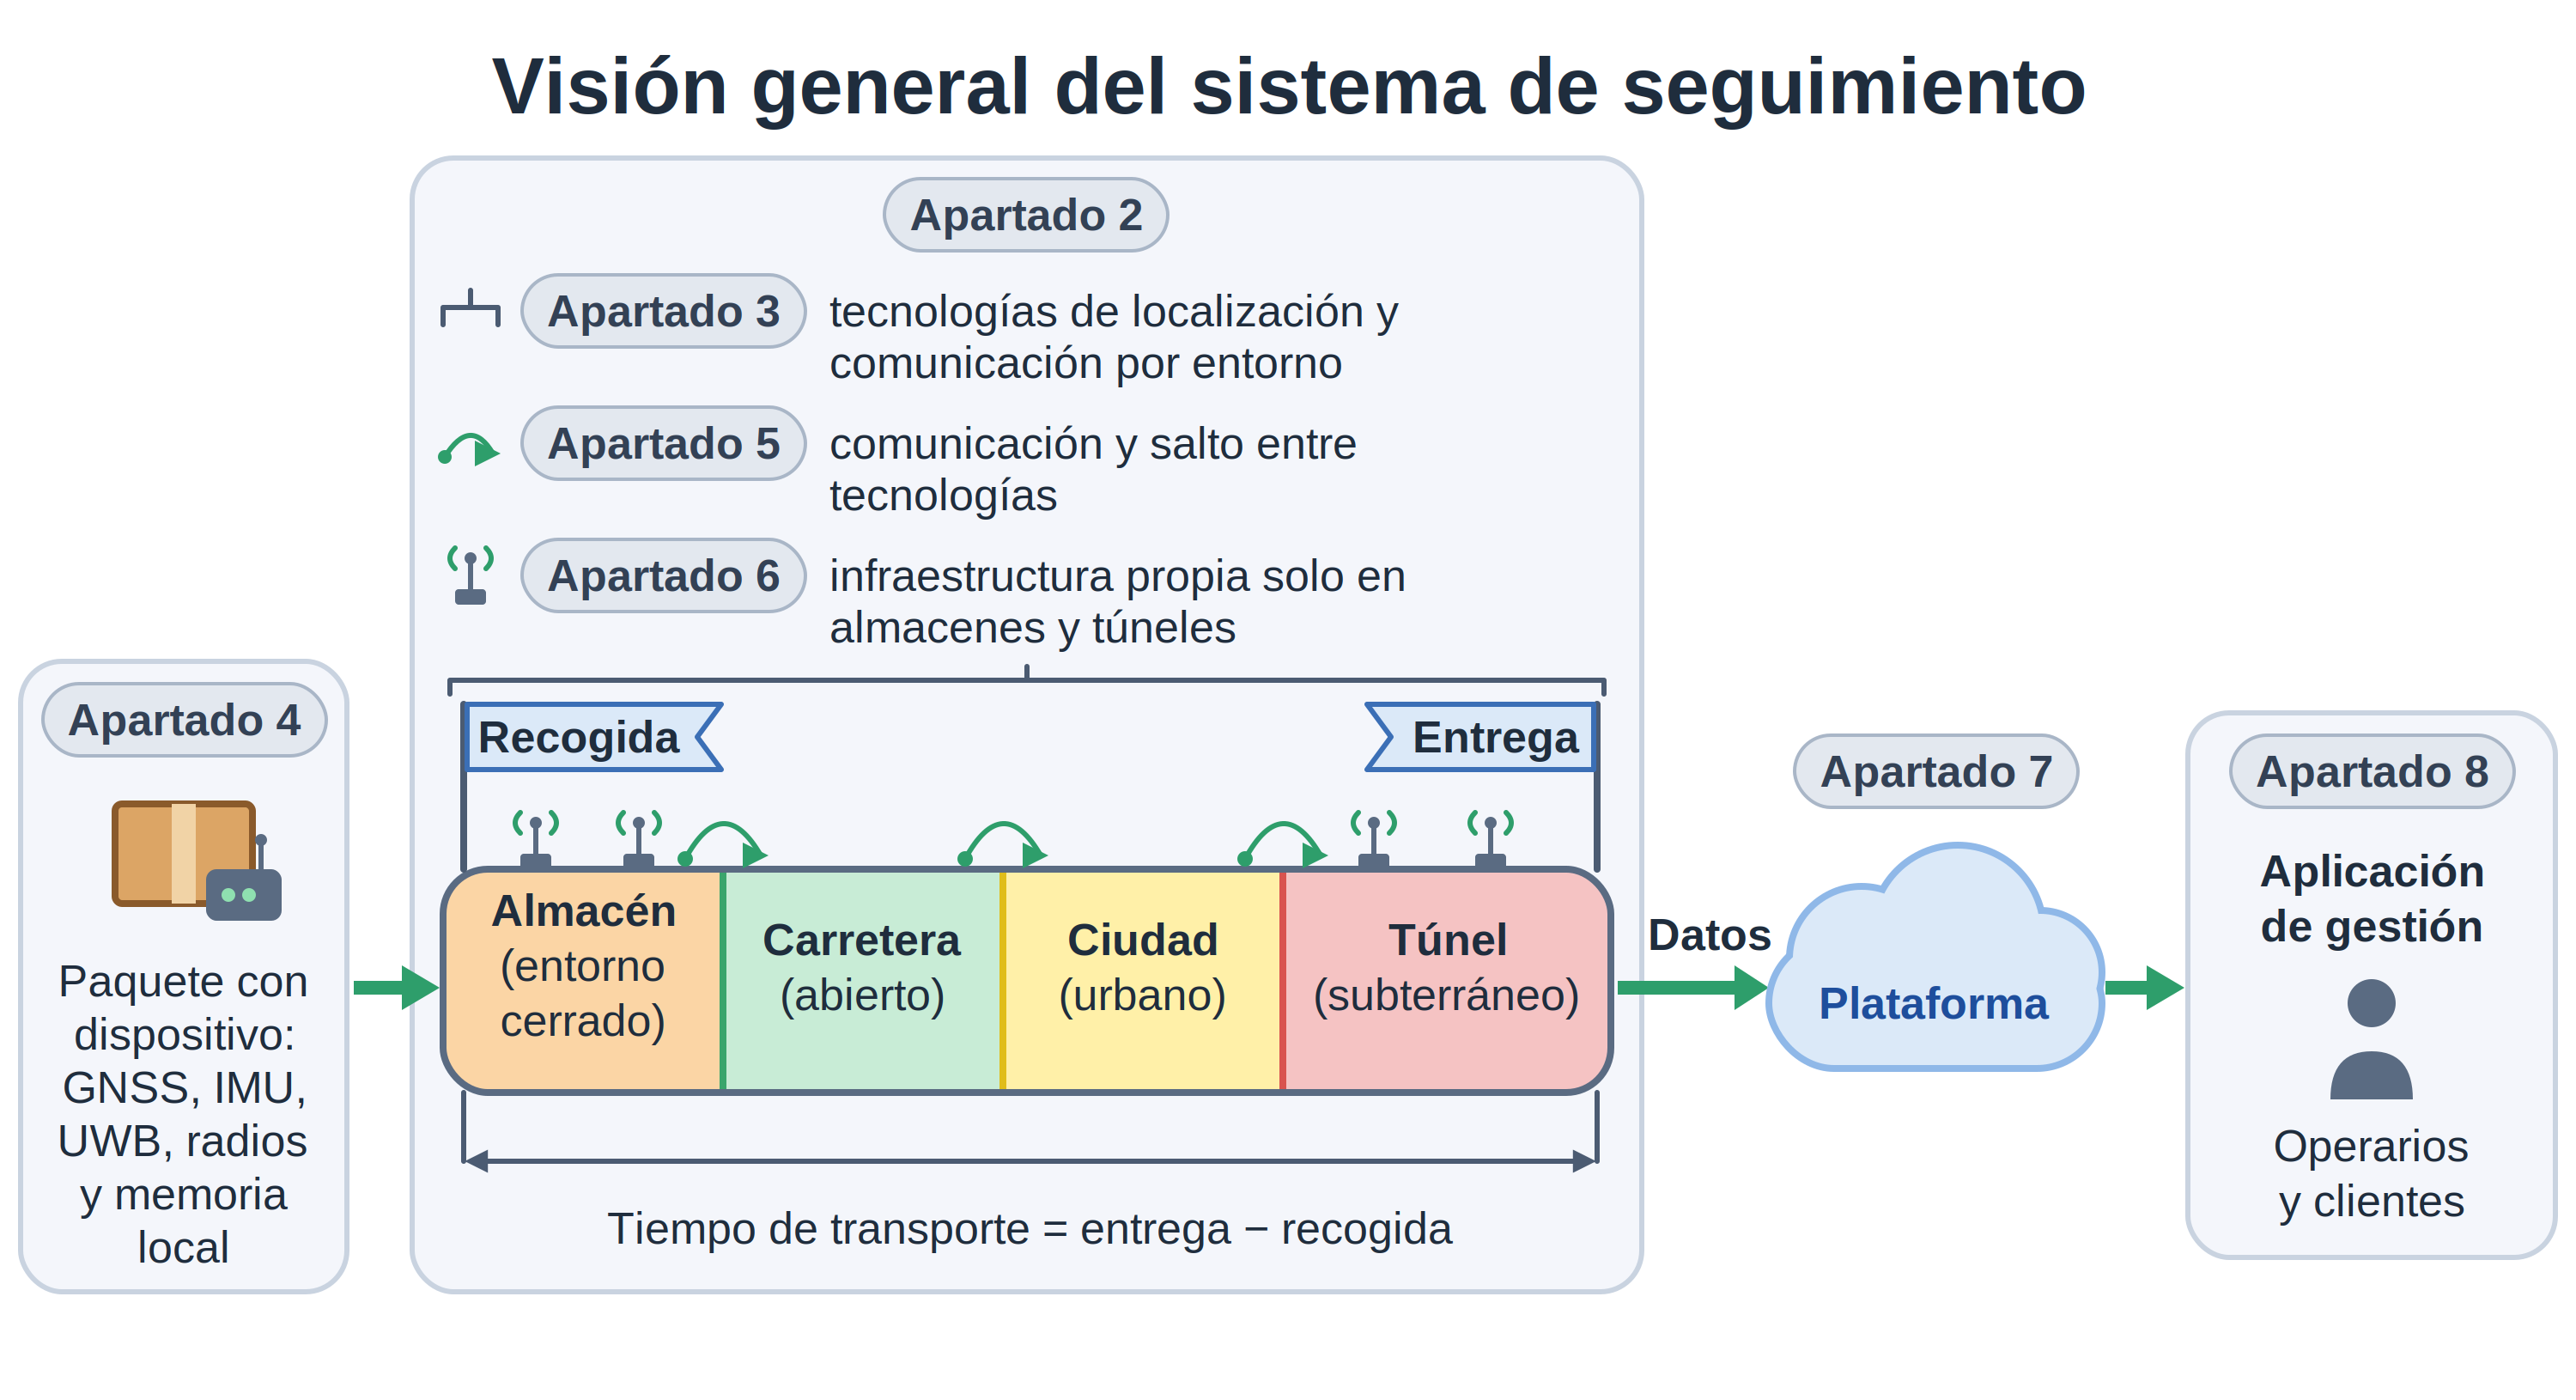
\includegraphics[width=\textwidth]{vision_general_sistema.png}
    \caption{Visión general del sistema de seguimiento propuesto, desde la recogida hasta la entrega.}
    \label{fig:vision_general}
\end{figure}

Buscamos con este trabajo ofrecer una solución integral, flexible y adaptable a los distintos entornos de transporte, que permita mejorar la trazabilidad de los paquetes y ofrecer información fiable sobre su recorrido y tiempos de entrega.

% =================================================================
% 2. CRITERIOS Y ENTORNOS
% =================================================================
\clearpage
\section{¿Qué criterios diferencian los distintos entornos por los que pasa el paquete?}
\label{sec:apartado2}

\subsection{Criterios para diferenciar los distintos entornos}
\label{sec:apartado2_1}

Para diseñar un sistema de seguimiento de paquetes es necesario identificar los entornos por los que circulan, ya que sus características físicas y radioeléctricas condicionan cómo se puede localizar el paquete y cómo se pueden transmitir sus datos.

Los criterios que se proponen para diferenciar los entornos por lo que pasa el paquete son los siguientes:

\begin{itemize}
    \item \textbf{Disponibilidad de señal del Global Navigation Satellite System (GNSS):} es el criterio principal que determina si es posible obtener la posición mediante sistemas como el Global Positioning System (GPS) o Galileo. En cielo abierto un receptor bien diseñado alcanza errores de unos pocos metros~\cite{ref1}, pero los edificios y las estructuras subterráneas pueden bloquear o degradar estas señales~\cite{ref2,ref3}, y en el interior de los túneles deja de ser una fuente fiable.

    \item \textbf{Cobertura de comunicaciones:} indica si existen redes móviles (2G/3G/4G/5G) con tecnologías como Narrowband Internet of Things (NB-IoT) o inalámbricas como Long Range Wide Area Network (LoRaWAN) y Wi-Fi, que permitan transmitir los datos a la plataforma de gestión. Estas tecnologías difieren en alcance, consumo y dependencia de un operador~\cite{ref4}, y en los túneles hay que tener en cuenta la ausencia de cobertura.

    \item \textbf{Obstáculos físicos y geometría:} los edificios, las paredes, las estanterías metálicas y los túneles pueden atenuar las señales y dificultar la localización~\cite{ref5}. En naves con mucho metal se generan muchas reflexiones~\cite{ref6} y en los túneles la propagación se comporta con una atenuación que depende de la frecuencia y las dimensiones del túnel~\cite{ref7}.

    \item \textbf{Infraestructura disponible:} se refiere a la existencia de antenas, puntos de acceso, lectores o balizas, así como la posibilidad de instalar nuevos elementos.

    \item \textbf{Movilidad:} considera la velocidad y las características del desplazamiento del paquete, desde el transporte por carretera hasta las operaciones de manipulación en almacenes.

    \item \textbf{Precisión y continuidad de la localización:} determinan el nivel de detalle necesario y si se requiere conocer la posición continuamente o solo en determinados puntos.

    \item \textbf{Autonomía energética y condiciones ambientales:} contemplan el consumo de los dispositivos, la duración del trayecto, la temperatura, la humedad y las vibraciones.
\end{itemize}

Estos criterios nos van a permitir identificar las limitaciones de cada entorno y establecer los requisitos que deberá cumplir el sistema de seguimiento.

\subsection{Clasificación propuesta de los entornos}
\label{sec:apartado2_2}

Se pueden distinguir cuatro entornos principales:

\begin{itemize}
    \item \textbf{Entorno abierto:} carreteras y autopistas. Presentan generalmente buena recepción GNSS y cobertura móvil. La localización geográfica suele ser viable sin desplegar infraestructura específica~\cite{ref8}.

    \item \textbf{Entorno urbano:} calles, y zonas industriales. Los edificios pueden bloquear o reflejar las señales, reduciendo la precisión del posicionamiento~\cite{ref9}. La cobertura de comunicaciones también puede variar según la zona.

    \item \textbf{Entorno cerrado:} almacenes y centros logísticos. La señal GNSS suele ser insuficiente o inexistente~\cite{ref10}. Las paredes, las estanterías y la maquinaria afectan a la propagación, por lo que puede ser necesario utilizar infraestructura de localización interior.

    \item \textbf{Entorno subterráneo:} túneles. La señal GNSS normalmente no está disponible y, según el enunciado del trabajo, tampoco existen comunicaciones. Por tanto, será necesario estudiar soluciones específicas para localizar el paquete y transmitir sus datos al exterior~\cite{ref11}.
\end{itemize}

\subsection{Relación criterios y entorno}
\label{sec:apartado2_3}

En la Tabla~\ref{tab:criterios_entornos} se relacionan los criterios anteriores con cada uno de los cuatro entornos.

\begin{table}[H]
    \centering
    \footnotesize
    \renewcommand{\arraystretch}{1.15}
    \begin{tabular}{@{}L{3.0cm}L{2.3cm}L{2.4cm}L{3.0cm}L{3.5cm}@{}}
        \toprule
        \textbf{Criterio} & \textbf{Carretera abierta} & \textbf{Entorno urbano} & \textbf{Almacén} & \textbf{Túnel} \\
        \midrule
        Señal GNSS & Buena & Variable & Generalmente inexistente & Inexistente o no utilizable \\
        Cobertura de comunicaciones & Disponible & Variable & Depende de infraestructura & No disponible \\
        Obstáculos físicos & Escasos & Edificios & Paredes y estanterías & Roca y hormigón (espacio confinado) \\
        Infraestructura adicional & Generalmente innecesaria & Puntualmente necesaria & Normalmente necesaria & Necesaria \\
        Movilidad & Alta & Media & Baja & Media \\
        Precisión & Tramo de vía & Calle y portal & Zona, pasillo o muelle & Tramo o posición en túnel \\
        Condiciones ambientales & Intemperie & Intemperie & Condiciones controladas & Humedad y polvo \\
        Principal dificultad & Continuidad de cobertura & Degradación de señales & Localización interior & Ausencia de GNSS y comunicaciones \\
        \bottomrule
    \end{tabular}
    \caption{Relación entre los criterios de diferenciación y los cuatro entornos del recorrido.}
    \label{tab:criterios_entornos}
\end{table}

En conclusión, las condiciones de localización y comunicación varían a lo largo del recorrido. Por ello, el sistema deberá adaptarse a cada entorno y contemplar especialmente los tramos en los que no sea posible obtener una posición mediante GNSS o transmitir los datos de forma directa. En los siguientes apartados estudiamos las tecnologías y sensórica que se utiliza en cada entorno, tal y como se ilustra en la Figura~\ref{fig:entornos}.

\begin{figure}[H]
    \centering
    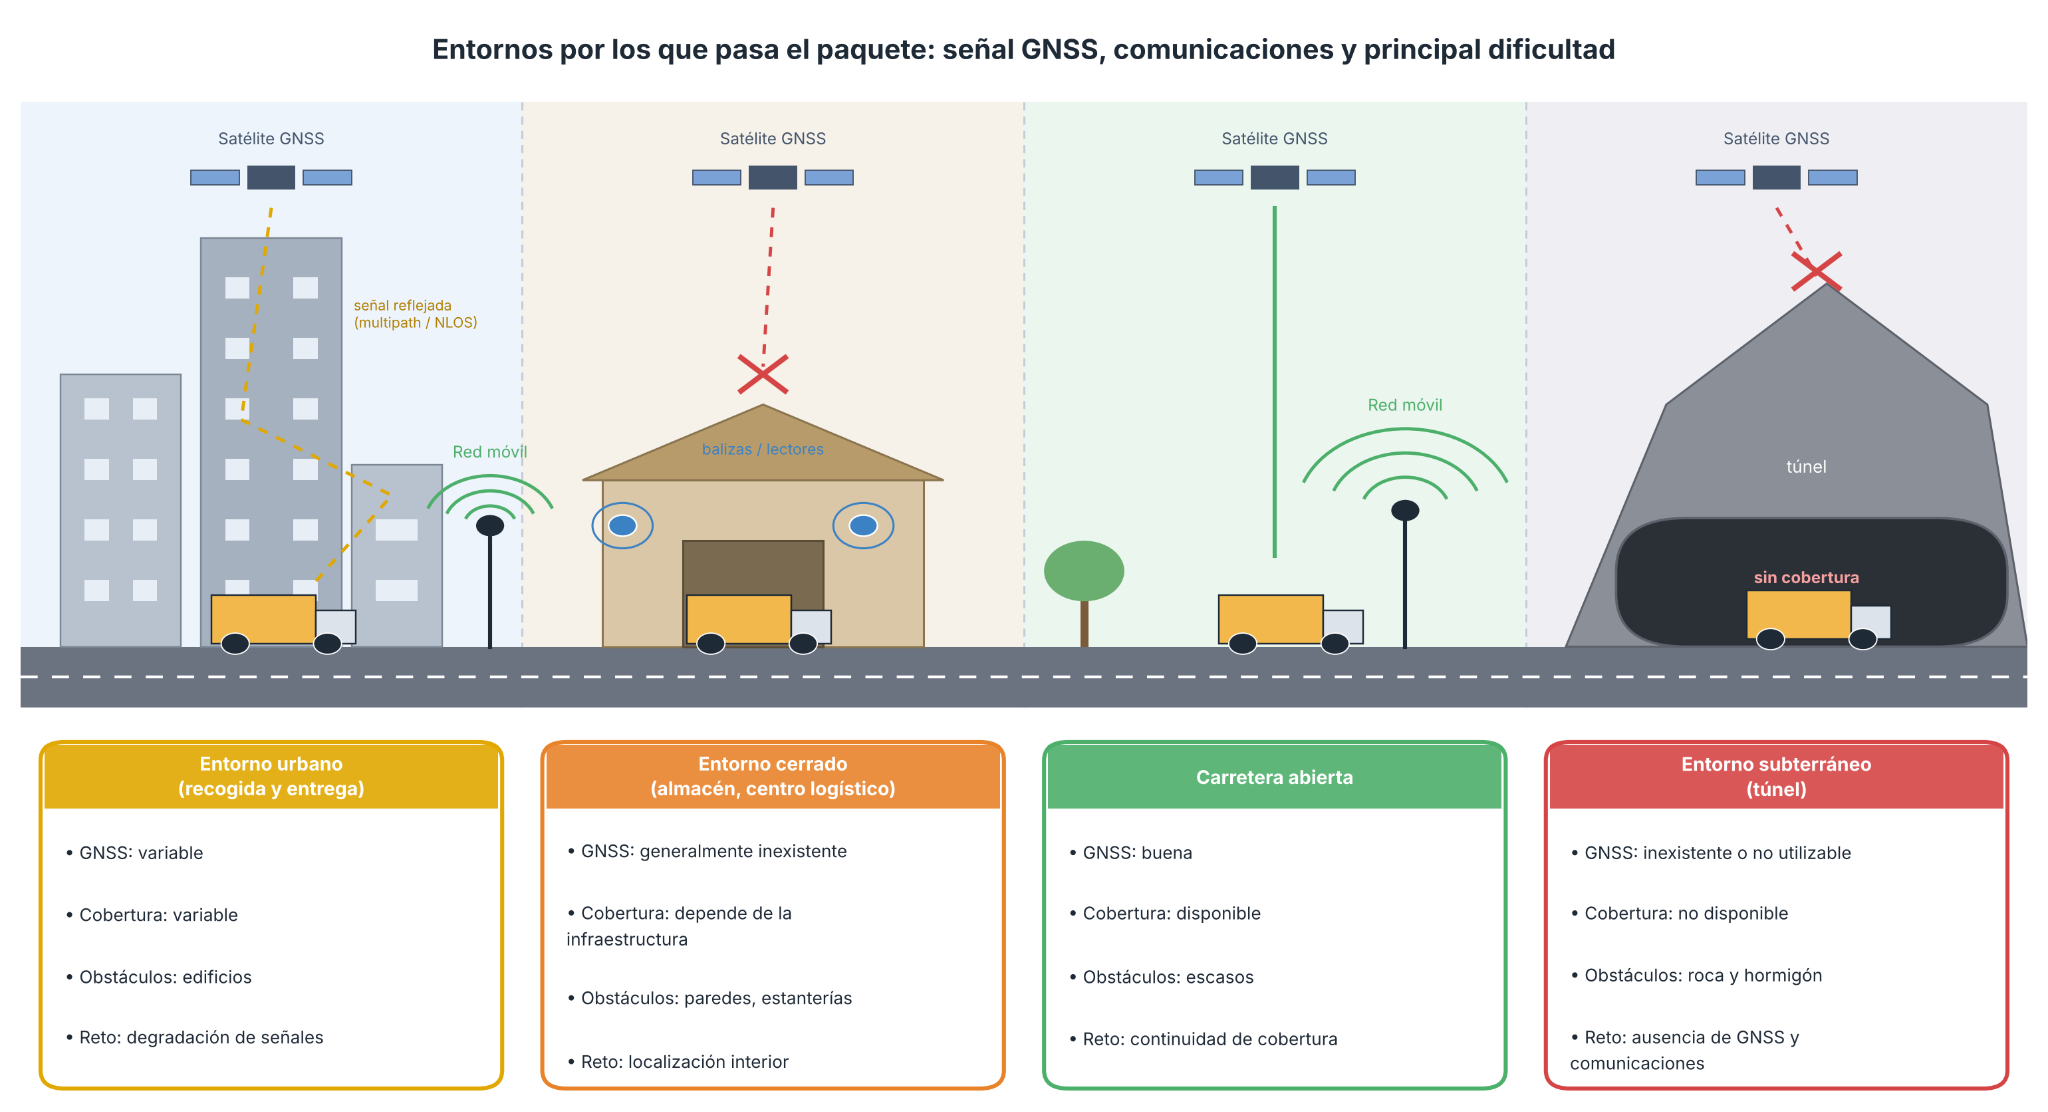
\includegraphics[width=\textwidth]{entornos.png}
    \caption{Entornos por los que pasa el paquete: señal GNSS, comunicaciones y principal dificultad.}
    \label{fig:entornos}
\end{figure}

% =================================================================
% 3. TECNOLOGÍAS POR ENTORNO
% =================================================================
\clearpage
\section{¿Qué tecnologías tendría que emplear en cada entorno?}
\label{sec:apartado3}

\subsection{Requisitos de comunicación y localización}
\label{sec:apartado3_1}

Para escoger las tecnologías con las que localizar el paquete y transmitir sus datos partimos de los criterios y de la clasificación de entornos definidos en la Sección~\ref{sec:apartado2}. De esto se pueden definir dos escenarios que se complementan. El de la localización, que responde a en qué punto del recorrido se encuentra el paquete, y el de las comunicaciones, que responde a cómo se hace llegar esa información a la plataforma de gestión. Los criterios de la Sección~\ref{sec:apartado2} (disponibilidad de señal GNSS, cobertura de comunicaciones, obstáculos físicos y geometría, infraestructura disponible, movilidad, precisión y continuidad de la localización y autonomía energética) condicionan ambos escenarios y nos permiten ordenar las tecnologías candidatas en cada entorno.

En el escenario de las comunicaciones las redes móviles y las tecnologías de red de área amplia de bajo consumo (Low-Power Wide-Area Network, LPWAN), en particular Long Term Evolution for Machines (LTE-M) y NB-IoT, ofrecen cobertura en espectro licenciado con bajo consumo y autonomías de varios años~\cite{ref12}. Además, LoRaWAN proporciona una arquitectura LPWA de extremo a extremo basada en puertas de enlace y pensada para dispositivos de bajo consumo~\cite{ref13}. Estas soluciones resultan adecuadas en los entornos abierto y urbano, donde la cobertura suele estar disponible aunque puede presentar huecos, pero en el interior de naves y túneles puede no existir, de modo que hay que desplegar infraestructura propia.

\subsection{Entorno abierto: carretera y autopista}
\label{sec:apartado3_2}

El entorno abierto es el más favorable para el seguimiento. Con cielo despejado, el GNSS proporciona por sí solo una posición válida sin necesidad de infraestructura adicional y si se emplean receptores de doble frecuencia o sistemas de aumentación, la precisión puede llegar a pocos centímetros~\cite{ref8}. Por ello se propone un receptor GNSS multiconstelación (por ejemplo GPS y Galileo) como fuente principal de localización y para reforzar la continuidad, la fusión con una unidad de medida inercial (IMU). La navegación inercial por sí sola acumula deriva con el tiempo y necesita correcciones periódicas del GNSS. Los esquemas de fusión IMU-GNSS mantienen una estimación razonable durante los cortes de señal y corrigen la deriva cuando la señal vuelve~\cite{ref14}.

Para las comunicaciones, este entorno dispone generalmente de cobertura móvil, aunque pueden existir tramos sin ella (la continuidad de cobertura que se señala en la Sección~\ref{sec:apartado2}), de modo que la vía natural es la red móvil 4G o 5G, complementada con las tecnologías LPWAN licenciadas LTE-M y NB-IoT cuando se prioricen el bajo consumo y el bajo coste frente al caudal~\cite{ref12}. Para un paquete en movimiento conviene priorizar LTE-M frente a NB-IoT, ya que LTE-M está mejor adaptada a aplicaciones con movilidad~\cite{ref15}. Como alternativa en espectro no licenciado puede considerarse LoRaWAN~\cite{ref13}. La propuesta en carretera es por tanto GNSS asistido por inercia para la posición y red móvil como vía principal de datos, reservando LoRaWAN para escenarios de bajo caudal.

\subsection{Entorno urbano}
\label{sec:apartado3_3}

El entorno urbano está en una posición intermedia. La localización por satélite sigue siendo la base pero los edificios bloquean o reflejan las señales y aparecen efectos de multitrayecto y de recepción sin línea de visión directa que deterioran la medida~\cite{ref2,ref8}. Por eso se propone reforzar el receptor GNSS con medidas en doble frecuencia. La señal L5 tiene un chip más corto que la L1 y reduce el error de multitrayecto hasta diez veces y su integración con técnicas asistidas por un modelo 3D del entorno (3D Mapping-Aided GNSS, 3DMA GNSS) permite alcanzar una precisión media del orden de 10~m en cañones urbanos~\cite{ref16}. La fusión con la IMU vuelve a ser útil para mantener la continuidad en las transiciones~\cite{ref14}.

En comunicaciones, la cobertura móvil suele estar disponible aunque puede variar de una calle a otra. Las tecnologías LTE-M y NB-IoT en espectro licenciado ofrecen buena cobertura tanto en interior como en exterior y están pensadas para mensajes breves y dispositivos de bajo consumo~\cite{ref12}. Se mantiene entonces la red móvil como método principal y se deja LoRaWAN como respaldo en zonas de cobertura débil~\cite{ref13}.

\subsection{Entorno cerrado: almacenes y centros logísticos}
\label{sec:apartado3_4}

En almacenes y centros logísticos la señal GNSS es insuficiente o inexistente, por lo que hay que desplegar infraestructura de localización interior~\cite{ref2,ref10}. Existen varias tecnologías candidatas con compromisos distintos entre precisión, alcance y coste.

La tecnología de banda ultra ancha (Ultra-Wideband, UWB) se caracteriza por usar mucho ancho de banda, por eso distingue la señal directa de los rebotes. Su rendimiento depende del ancho de banda, la frecuencia central y el material de construcción~\cite{ref17}.

Para las comunicaciones se propone aprovechar la red local del almacén (Wi-Fi o Ethernet) y cuando se necesite bajo consumo y cobertura amplia dentro del recinto, LoRaWAN con puertas de enlace propias~\cite{ref13}. La Tabla~\ref{tab:localizacion_interior} compara las alternativas de localización interior.

\begin{table}[H]
    \centering
    \footnotesize
    \renewcommand{\arraystretch}{1.15}
    \begin{tabular}{@{}L{3.0cm}L{6.9cm}L{4.0cm}@{}}
        \toprule
        \textbf{Tecnología} & \textbf{Prestaciones} & \textbf{Uso propuesto} \\
        \midrule
        UWB & Resolución temporal muy fina para resolver el multitrayecto~\cite{ref17} & Localización fina en la nave \\
        Wi-Fi RTT (Round-Trip Time) & Basada en el estándar 802.11. 1--2~m con tres o más puntos de acceso~\cite{ref18} & Reutilizar la red inalámbrica existente \\
        Bluetooth Channel Sounding & Combina medida de fase y tiempo de ida y vuelta. Desde 50~cm hasta 100~m~\cite{ref19} & Equilibrio entre coste y precisión \\
        \bottomrule
    \end{tabular}
    \caption{Comparación de las alternativas de localización interior en almacenes.}
    \label{tab:localizacion_interior}
\end{table}

Se considera que UWB es la opción más precisa cuando se puede asumir el coste de su infraestructura. Wi-Fi RTT y Bluetooth Channel Sounding se contemplan como alternativas teóricas analizadas para el caso de que la nave ya dispusiera de dicha infraestructura inalámbrica y se buscase evitar el despliegue de anclas UWB.

\subsection{Entorno subterráneo: túneles}
\label{sec:apartado3_5}

En los túneles no hay GNSS y según el enunciado tampoco comunicaciones, por lo que tanto la localización como la transmisión dependen por completo de infraestructura propia. La propagación en este entorno es singular. La Recomendación ITU-R P.1406 (International Telecommunication Union -- Radiocommunication Sector, ITU-R) trata los efectos de propagación en servicios móviles terrestres y de radiodifusión en las bandas de VHF y UHF y dedica un apartado específico a la propagación guiada en túneles y a los cables radiantes~\cite{ref9}. Además, el comportamiento depende de la geometría del túnel y de las propiedades eléctricas de sus paredes, por lo que se necesitan modelos de propagación específicos para túneles~\cite{ref7}.

Para las comunicaciones, el cable radiante (\emph{leaky feeder}) se utiliza en minas subterráneas, donde en muchos casos puede ser la única vía para transportar los datos de monitorización~\cite{ref20}. Además, se ha comprobado que LoRa, operando en la banda de 868~MHz, se propaga en minas subterráneas de sal con un comportamiento cuasi guía de onda, lo que permite enlaces sin línea de visión superiores a 1000~m con una pérdida de paquetes inferior al 15\,\%~\cite{ref21}.

En un túnel real de 2,4~km de longitud, se comprobó que una única puerta de enlace situada en la entrada es suficiente para proporcionar cobertura en todo el recinto~\cite{ref22}. No obstante, dado que dicho ensayo se realizó en un único entorno y sin tráfico, se propone el despliegue de un cable radiante a lo largo de la infraestructura como columna vertebral de las comunicaciones; esto ofrece un mayor margen de enlace y elimina la dependencia de la posición del dispositivo. Como complemento, se plantean nodos LoRa en los puntos donde el tendido de cable no sea viable, mientras que en túneles de longitud similar, la cobertura inalámbrica desde la entrada podría bastar como una alternativa más sencilla.

Cuando se combina UWB con una IMU, como en el caso de una mina de carbón subterránea, los errores de posición pueden controlarse por debajo de 0,1~m, y el sistema inercial cubre los cortes de señal de UWB~\cite{ref23}. Por tanto se propone UWB asistido por inercia para la posición dentro del túnel y cable radiante con apoyo de LoRa para enviar los datos al exterior, como se representa en la Figura~\ref{fig:tunel}.

\begin{figure}[H]
    \centering
    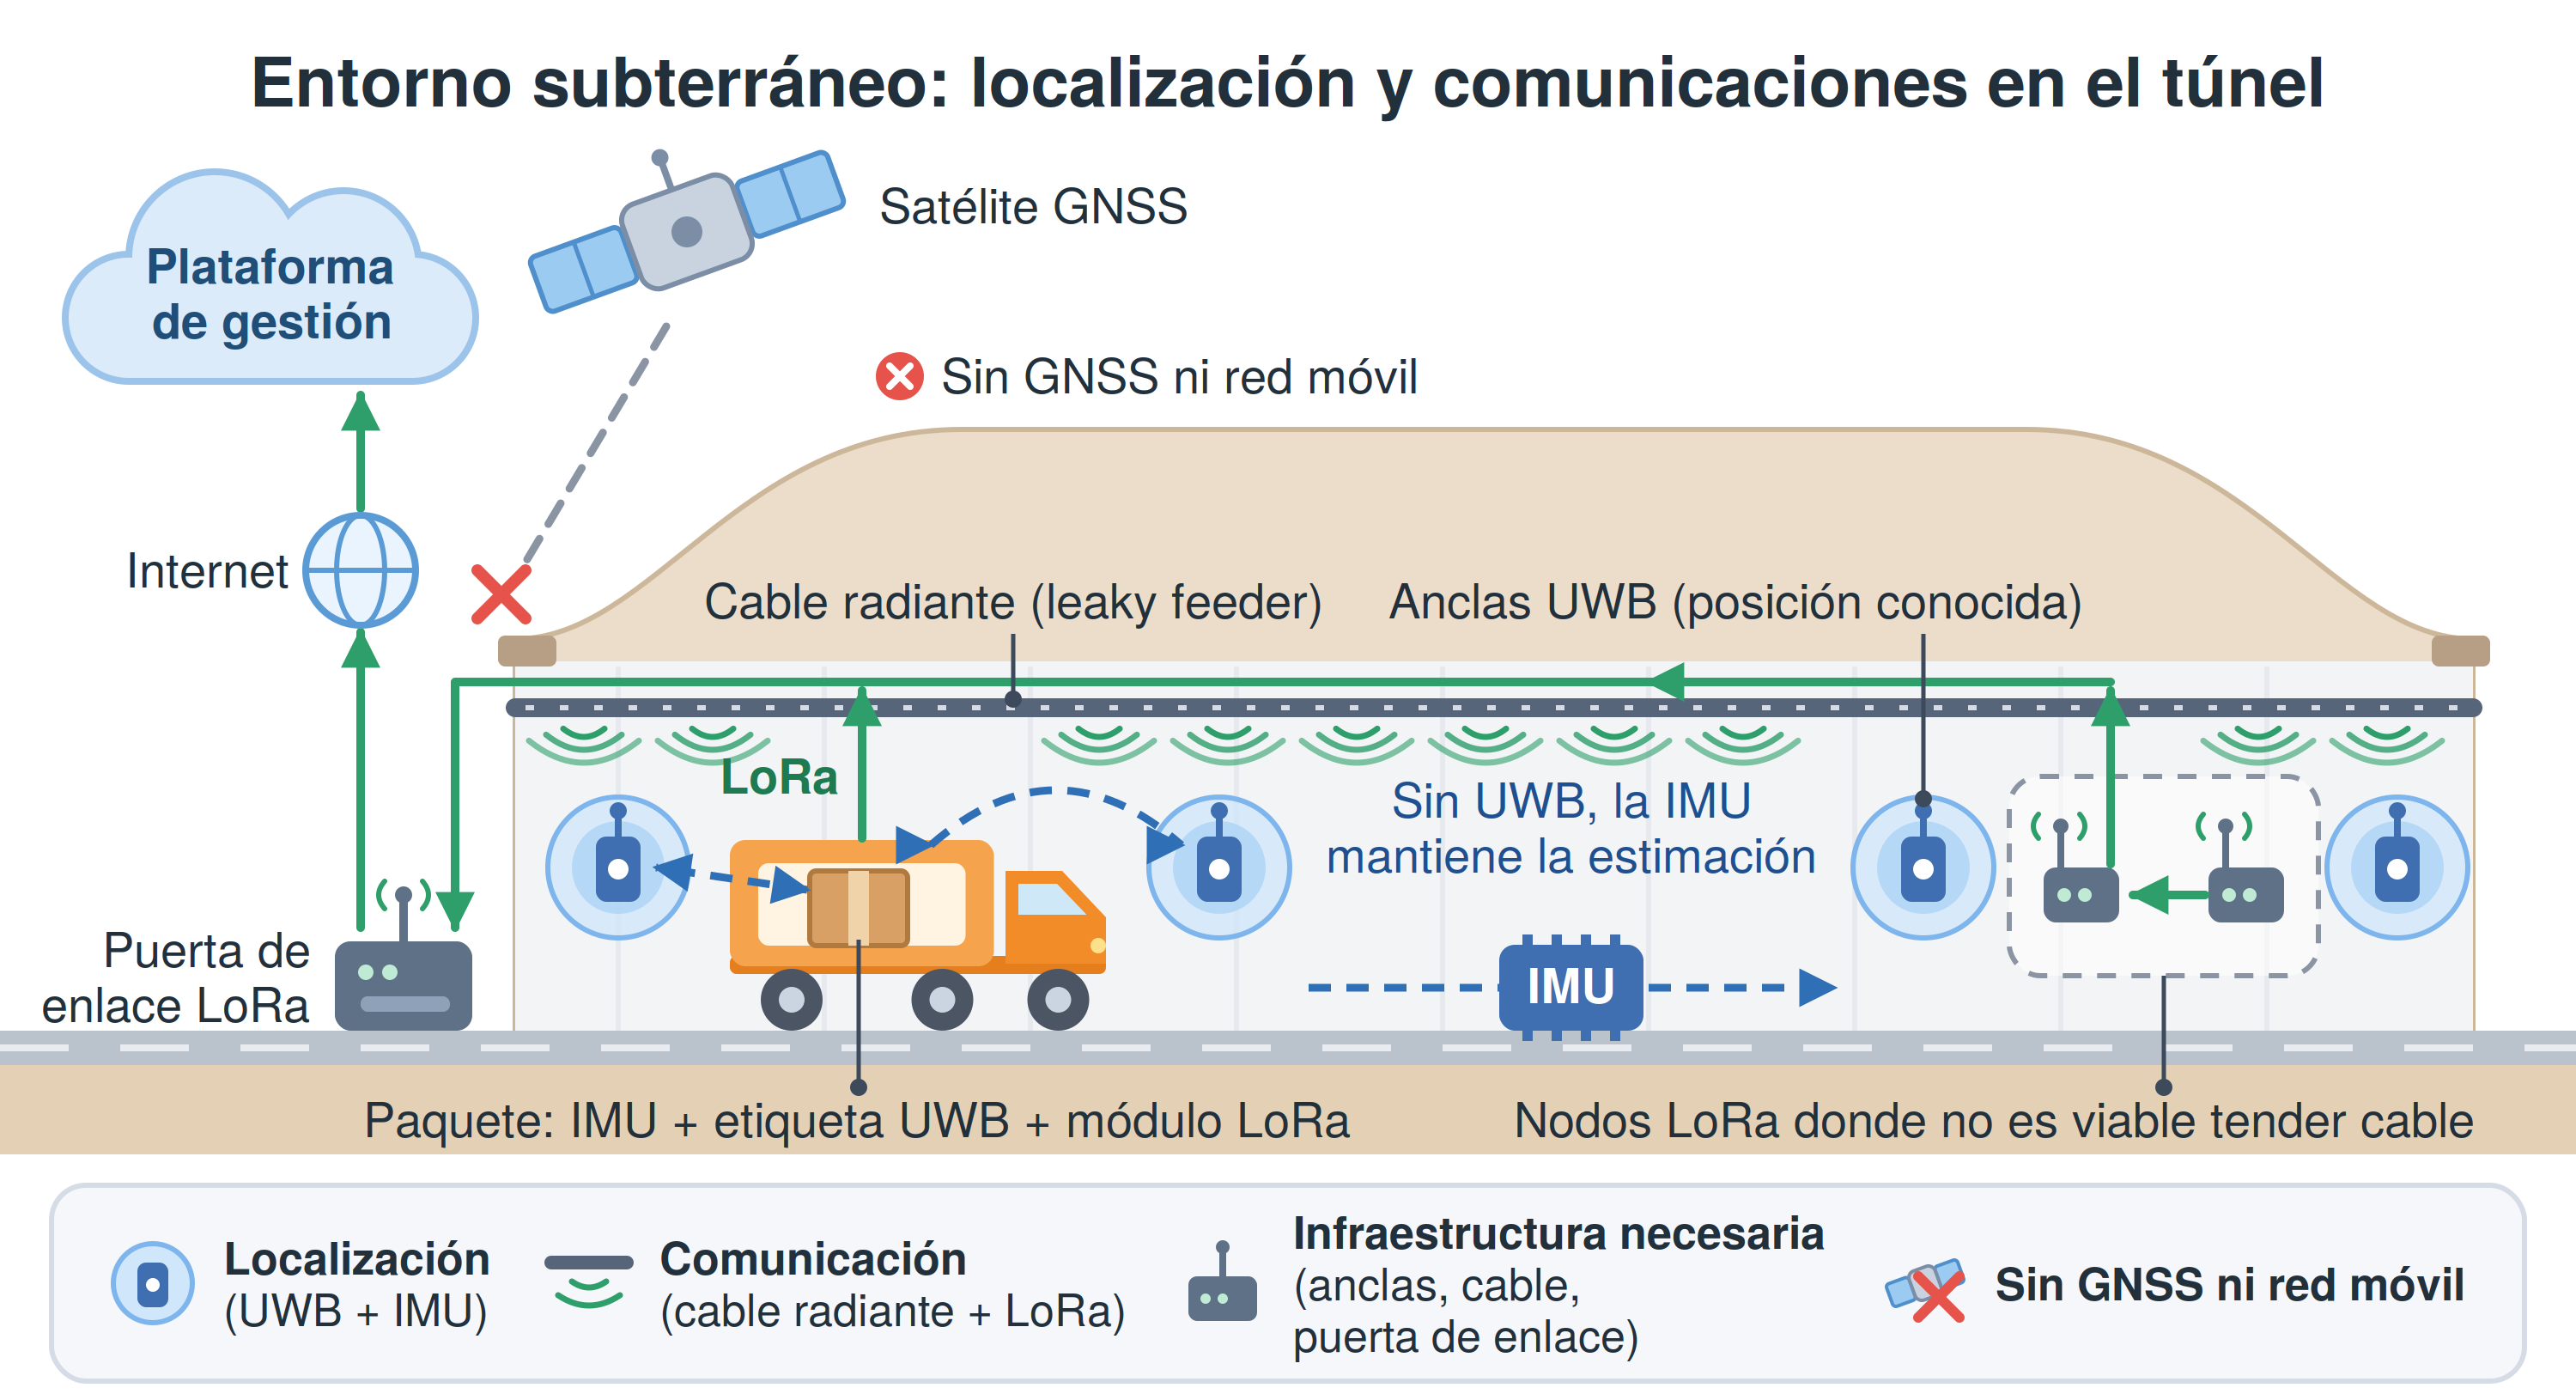
\includegraphics[width=\textwidth]{tunel_localizacion_comunicaciones-2.png}
    \caption{Entorno subterráneo: localización y comunicaciones en el túnel.}
    \label{fig:tunel}
\end{figure}

\subsection{Resumen de tecnologías a emplear}
\label{sec:apartado3_6}

La Tabla~\ref{tab:resumen_tecnologias} resume la propuesta tecnológica para cada entorno.

\begin{table}[H]
    \centering
    \footnotesize
    \renewcommand{\arraystretch}{1.15}
    \begin{tabular}{@{}L{3.2cm}L{5.2cm}L{6.2cm}@{}}
        \toprule
        \textbf{Entorno} & \textbf{Localización} & \textbf{Comunicación} \\
        \midrule
        Abierto (carretera y autopista) & GNSS multiconstelación con fusión IMU~\cite{ref8,ref14} & Red móvil 4G/5G; LTE-M y NB-IoT; LoRaWAN como alternativa~\cite{ref12,ref13} \\
        Urbano & GNSS en doble frecuencia L1/L5 con 3DMA y fusión IMU~\cite{ref14,ref16} & Red móvil; LoRaWAN de respaldo~\cite{ref12,ref13} \\
        Cerrado (almacenes) & UWB, Wi-Fi RTT o Bluetooth Channel Sounding~\cite{ref17,ref18,ref19} & Red local del recinto; LoRaWAN con puertas de enlace propias~\cite{ref13} \\
        Subterráneo (túneles) & UWB asistido por IMU~\cite{ref23} & Cable radiante con nodos LoRa~\cite{ref9,ref20,ref21} \\
        \bottomrule
    \end{tabular}
    \caption{Resumen de las tecnologías de localización y comunicación propuestas para cada entorno.}
    \label{tab:resumen_tecnologias}
\end{table}

Se considera que ninguna tecnología aislada cubre todo el recorrido, sino que se trata de una combinación complementaria: el GNSS resuelve el exterior, la banda ultra ancha y las redes inalámbricas de corto alcance resuelven el interior, y el cable radiante con apoyo de LoRa resuelve el túnel. Para que el paquete no pierda trazabilidad al cambiar de entorno habrá que prever la transición entre tecnologías, aspecto que se desarrolla en la Sección~\ref{sec:apartado5}, y dotar al paquete de los sensores descritos en la Sección~\ref{sec:apartado4}. Los elementos externos que materializan esta infraestructura, como antenas, anclas y nodos, se abordan en la Sección~\ref{sec:apartado6}, correspondiente al despliegue de antenas.

% =================================================================
% 4. SENSORES DEL PAQUETE
% =================================================================
\clearpage
\section{¿Qué sensores debería incluirse en los paquetes junto con las necesidades operativas y las necesidades para comunicarse con las distintas tecnologías?}
\label{sec:apartado4}

Cada paquete llevará un dispositivo con identificador único, sensores, módulos de localización y radios para transmitir los datos. Un microcontrolador coordinará estos elementos, junto con una batería, un reloj y memoria no volátil. La arquitectura del dispositivo descrito se muestra en la Figura~\ref{fig:dispositivo_paquete}.

\begin{figure}[H]
    \centering
    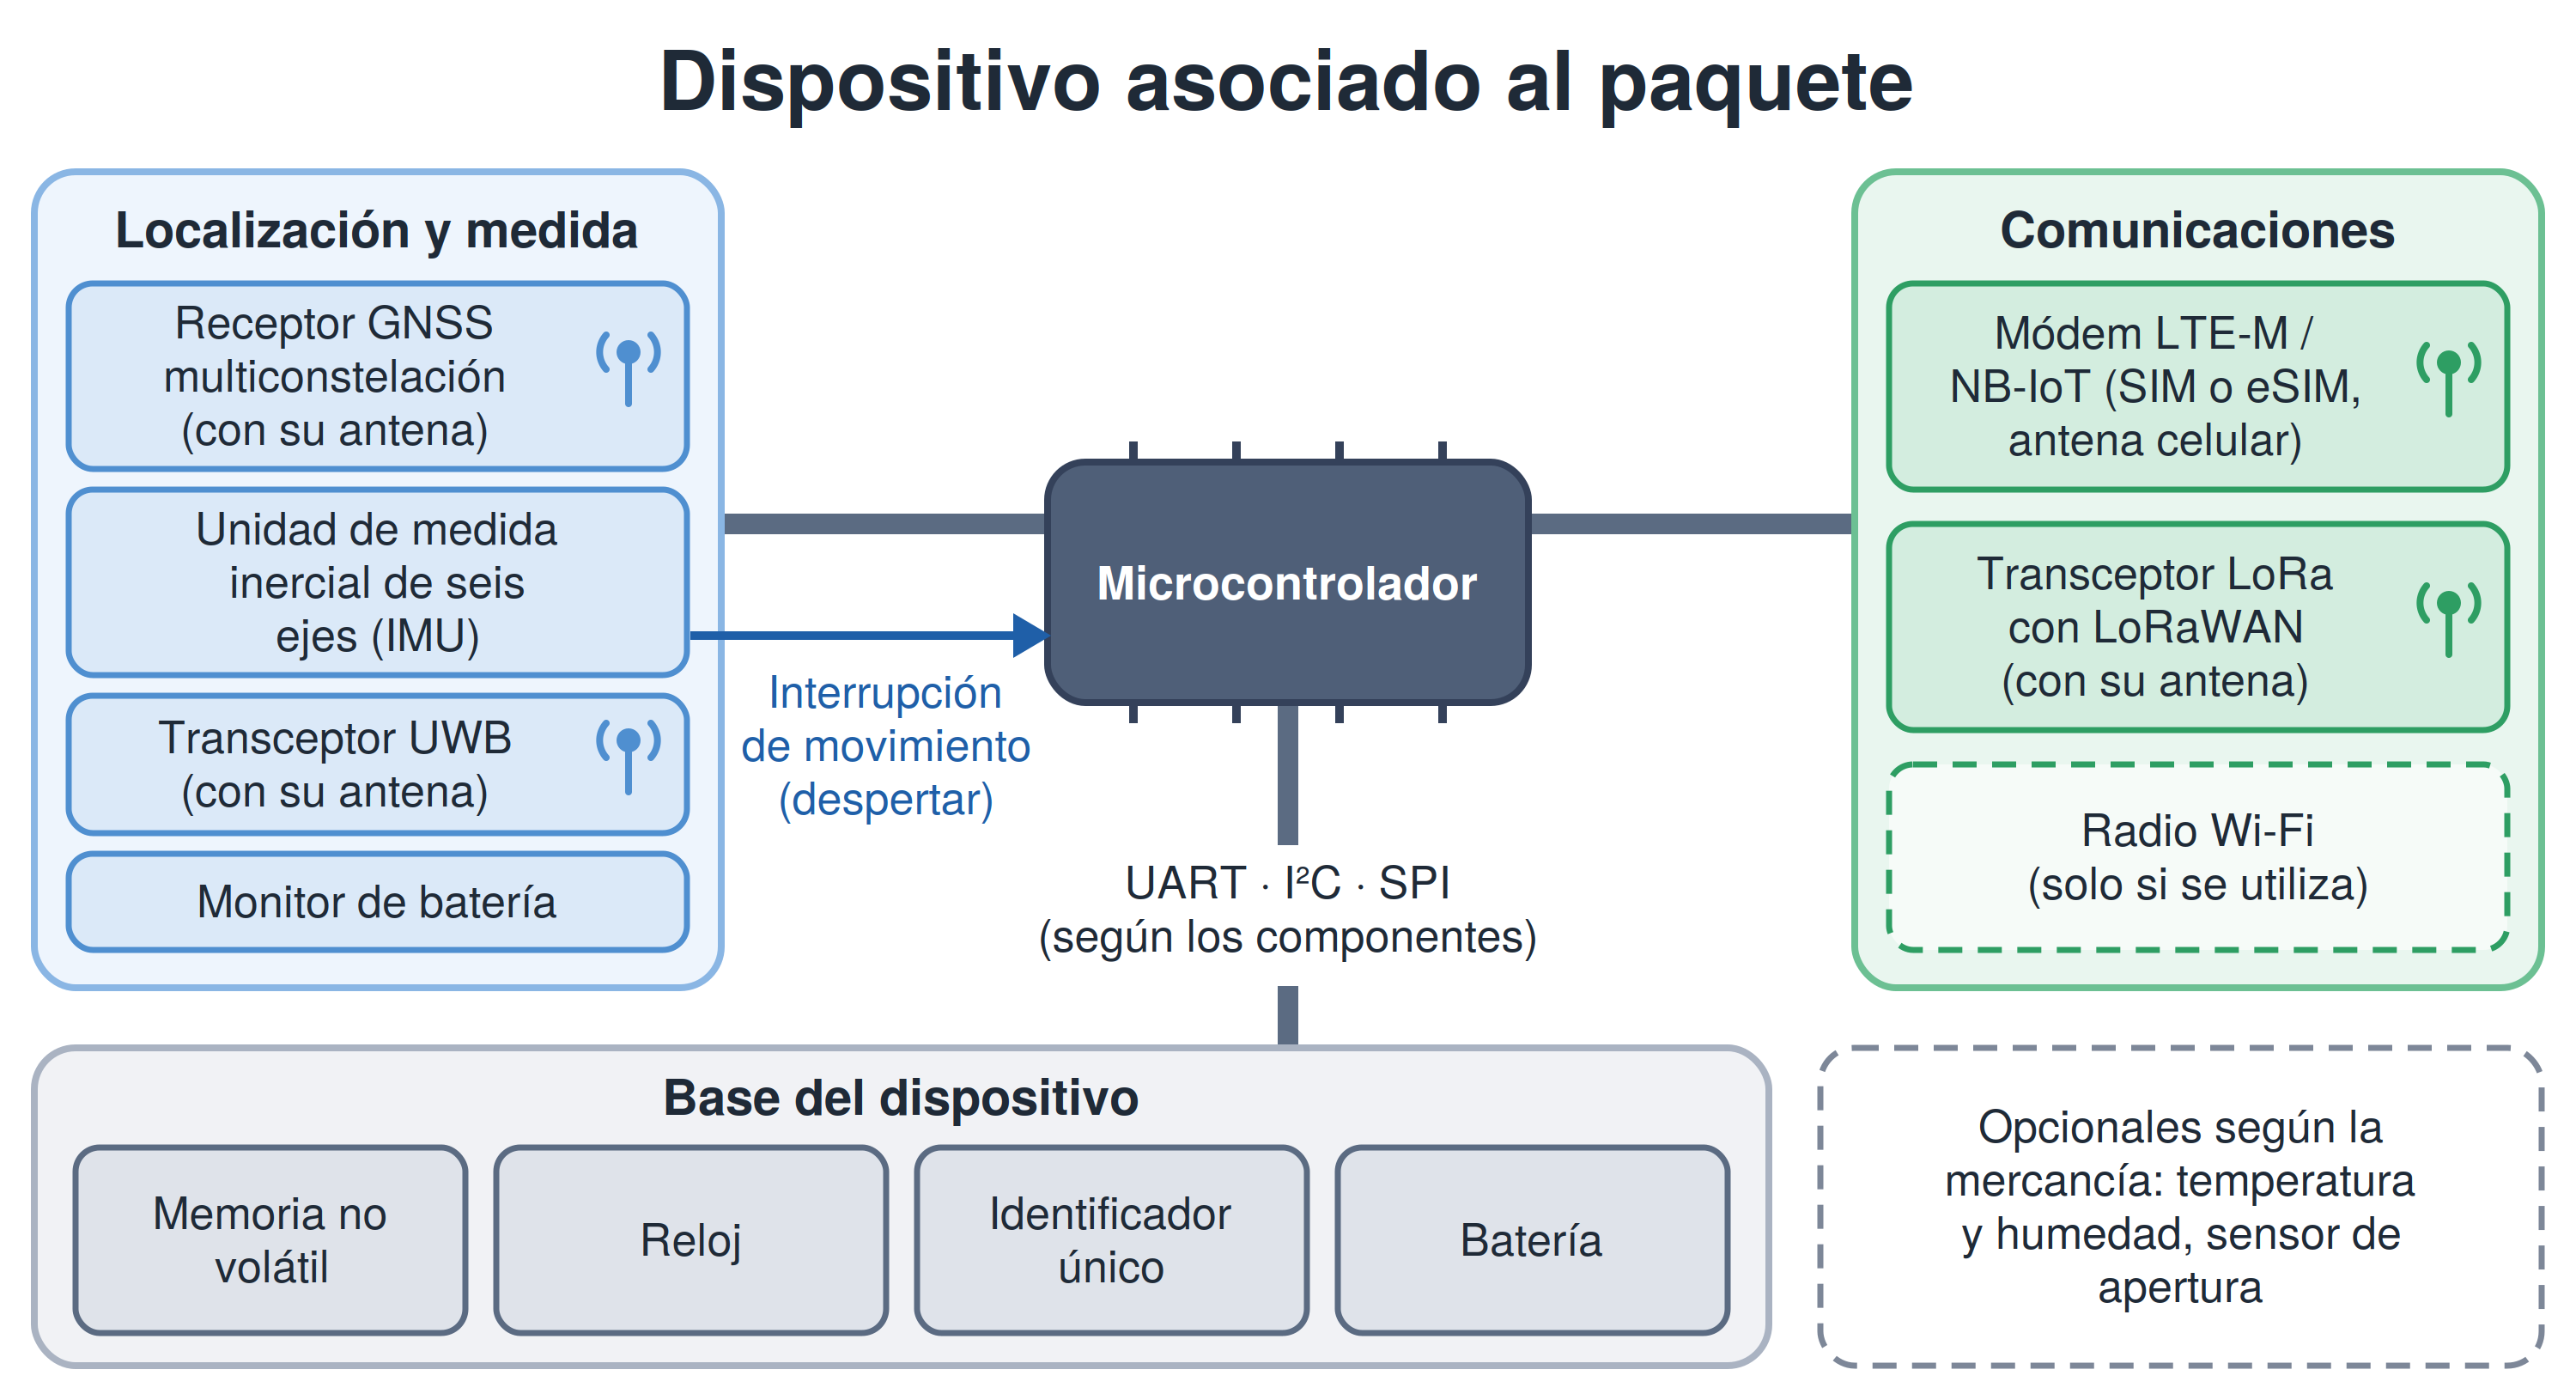
\includegraphics[width=\textwidth]{dispositivo_paquete_bloques.png}
    \caption{Dispositivo asociado al paquete: sensores, módulos de localización, comunicaciones y base del dispositivo.}
    \label{fig:dispositivo_paquete}
\end{figure}

\subsection{Sensores y elementos de localización}
\label{sec:apartado4_1}

En la Tabla~\ref{tab:sensores} se detallan los sensores y elementos de localización que incorpora el dispositivo.

\begin{table}[H]
    \centering
    \footnotesize
    \renewcommand{\arraystretch}{1.15}
    \begin{tabular}{@{}L{3.7cm}L{5.1cm}L{5.8cm}@{}}
        \toprule
        \textbf{Elemento} & \textbf{Función} & \textbf{Requisitos} \\
        \midrule
        GNSS multiconstelación & Localizar en exteriores. & Antena con recepción suficiente, doble frecuencia y soporte SBAS/EGNOS. \\
        IMU de seis ejes & Medir aceleraciones y giros; detectar movimiento. & Fijación y calibración. Corregir la deriva con GNSS o UWB. \\
        Transceptor UWB & Localizar en almacenes y túneles. & Anclas de posición conocida y configuración compatible. \\
        Monitor de batería & Medir la carga disponible. & Aviso de batería baja antes de perder el seguimiento. \\
        \bottomrule
    \end{tabular}
    \caption{Sensores y elementos de localización del dispositivo asociado al paquete.}
    \label{tab:sensores}
\end{table}

\subsection{Necesidades operativas}
\label{sec:apartado4_2}

La batería deberá cubrir el envío y los posibles retrasos. Para ahorrar energía, se espaciarán las actualizaciones en reposo y se desactivarán los módulos innecesarios. Las frecuencias de medida y transmisión se ajustarán por separado según la autonomía y la capacidad de la red.

Cada registro conservará identificador, secuencia, marca de tiempo, posición, precisión estimada, fuente de localización, batería y el tipo de evento (como posición periódica, salida o entrada) y, si procede, el identificador del ancla leída, conforme al formato de la Sección~\ref{sec:apartado5_1}. El reloj utilizará una referencia temporal común y la memoria guardará los datos durante los cortes para reenviarlos al recuperar conexión.

La recogida y la entrega se registrarán explícitamente mediante escaneo y confirmación del operario. El tiempo de transporte será la diferencia entre ambas marcas temporales, independientemente de cuándo lleguen los datos a la plataforma. Los eventos automáticos de entrada y salida descritos en la Sección~\ref{sec:apartado5_2} no sustituyen a estos escaneos, sino que permiten desglosar ese tiempo total por etapas.

El dispositivo deberá resistir golpes, vibraciones, polvo y humedad, y quedar bien fijado. Las antenas se colocarán evitando el apantallamiento por vehículos o embalajes metálicos; la cobertura se comprobará con la carga real.

\subsection{Necesidades para comunicarse con las distintas tecnologías}
\label{sec:apartado4_3}

Se propone LTE-M como enlace móvil principal, con módem, antena y Subscriber Identity Module (SIM) o embedded SIM (eSIM) compatibles con el operador. LoRaWAN requerirá radio LoRa, antena, identificadores y claves, además de puertas de enlace conectadas al servidor de red~\cite{ref24}. Las credenciales deberán protegerse y los mensajes ajustarse a la capacidad de cada enlace.

En el túnel, la radio LoRa deberá ser compatible con la banda y los equipos asociados al cable radiante. El seguimiento en tiempo real dependerá de las anclas UWB y de una conexión hasta el exterior. En almacenes podrá añadirse Wi-Fi; si se elige Wi-Fi RTT o Bluetooth Channel Sounding, tanto el dispositivo como la infraestructura deberán admitir esas funciones~\cite{ref18,ref19}. Los buses y la conmutación se detallan en la Sección~\ref{sec:apartado5}.

% =================================================================
% 5. COMUNICACIÓN ENTRE COMPONENTES Y SALTO ENTRE TECNOLOGÍAS
% =================================================================
\clearpage
\section{¿Qué mecanismos se emplean para realizar la comunicación entre componentes y cómo realizar el salto entre distintas tecnologías?}
\label{sec:apartado5}

\subsection{Mecanismos de comunicación entre componentes}
\label{sec:apartado5_1}

La comunicación del sistema se produce en tres tramos distintos, cada uno con sus propios mecanismos: dentro del dispositivo, entre el dispositivo y la infraestructura de localización, y entre el dispositivo y la plataforma. Así evitamos confundir qué tecnología se usa en cada entorno, que ya se ha tratado en la Sección~\ref{sec:apartado3}, con cómo se comunican realmente los componentes entre sí.

\begin{itemize}
    \item \textbf{Dentro del dispositivo (sensores y módulos de radio con el microcontrolador):} el microcontrolador actúa como coordinador porque es el único componente que conoce el estado de todos los demás y puede decidir qué tecnología usar en cada momento (Sección~\ref{sec:apartado5_2}). Cada componente se conecta con el bus que mejor se adapta a los datos que mueve:
    \begin{itemize}
        \item \textbf{Receptor GNSS por UART:} entrega un flujo continuo y de poca velocidad de tramas de texto de la National Marine Electronics Association (NMEA) con la posición, y el puerto serie Universal Asynchronous Receiver-Transmitter (UART) es la interfaz que casi todos estos receptores incorporan.

        \item \textbf{IMU por I\textsuperscript{2}C o SPI:} entrega pocos datos pero con mucha frecuencia. Inter-Integrated Circuit (I\textsuperscript{2}C) usa solo dos hilos y permite compartirlos con otros sensores, y Serial Peripheral Interface (SPI) se elige si hace falta más velocidad.

        \item \textbf{Transceptor UWB y radio LoRa por SPI:} necesitan un bus rápido y de respuesta inmediata, el primero para medir tiempos de vuelo con precisión y el segundo para cargar y leer los mensajes.

        \item \textbf{Módem móvil por UART con comandos AT:} es la interfaz estándar de estos módems y evita programar la pila de red, que ya resuelve el propio módem.

        \item \textbf{Línea de interrupción de la IMU:} despierta al microcontrolador cuando detecta movimiento, de modo que el dispositivo permanece en reposo mientras el paquete está parado. Es necesario porque el consumo es la restricción principal de un dispositivo que no se puede recargar durante el transporte.
    \end{itemize}

    \item \textbf{Localización por satélite (GNSS):} el receptor GNSS multi-constelación (por ejemplo GPS y Galileo, en doble frecuencia en el entorno urbano) solo recibe las señales de los satélites y calcula la posición en el propio dispositivo. Al ser un enlace unidireccional no necesita ninguna infraestructura propia ni intercambio de mensajes con equipos externos, y por eso es la fuente preferida en el exterior.

    \item \textbf{Entre el dispositivo y la infraestructura de localización interior (UWB):} el dispositivo y los equipos UWB fijos (anclas) intercambian mensajes de medida de distancia mediante \emph{two-way ranging}, que mide el tiempo de ida y vuelta de la señal y está recogido en el estándar IEEE 802.15.4z~\cite{ref25}. Se mide el tiempo y no la intensidad de la señal porque la intensidad varía mucho con las reflexiones en superficies metálicas, muy habituales en almacenes y túneles, mientras que el tiempo permite precisión de decímetros combinando UWB con una IMU~\cite{ref23}. Se usa ida y vuelta, y no un solo sentido, porque así no hace falta que los relojes del dispositivo y del ancla estén sincronizados entre sí. Con las distancias a al menos tres anclas de posición conocida se calcula la posición en un plano por trilateración~\cite{ref17}, y con una cuarta también la altura. Si en el almacén se optara por Wi-Fi RTT o Bluetooth Channel Sounding, el principio es el mismo (medida del tiempo o de la fase de ida y vuelta con puntos de acceso o balizas de posición conocida~\cite{ref18,ref19}) y solo cambia la infraestructura. Este enlace se usa solo para localizar porque su alcance es de decenas de metros y no tiene salida a internet, de modo que los datos viajan por otro canal.

    \item \textbf{Entre el dispositivo y la plataforma (transporte de datos):} una vez obtenida la posición con la fuente activa, el microcontrolador la envía a la plataforma de forma periódica y también cuando ocurre un evento relevante, como la salida del almacén o la entrada en el túnel. La frecuencia de envío puede ser menor que la de medida, de modo que no todas las medidas se transmiten al instante. Para ello, la posición se empaqueta en un mensaje binario compacto de unos 20 bytes con el identificador del paquete, un número de secuencia, la marca de tiempo, las coordenadas, la precisión estimada, la tecnología de localización usada, el nivel de batería y el tipo de evento (como posición periódica, salida o entrada) y, si procede, el identificador del ancla leída. Se usa un formato binario, y no texto como JavaScript Object Notation (JSON) que ocuparía varias veces más, porque LoRaWAN limita el tamaño del mensaje y porque en la banda de 868~MHz de la UE el tiempo de emisión está limitado por el ciclo de trabajo, del 1\,\% en la mayoría de subbandas~\cite{ref26,ref27,ref28}. Cada dato tiene su motivo: el número de secuencia sirve para ordenar y detectar mensajes perdidos, la marca de tiempo para el estudio de tiempos, la precisión para que la plataforma sepa cuánto fiarse de la posición y la tecnología usada para poder explicar posibles diferencias. El contenido del mensaje es el mismo en todos los canales, por lo que lo llamaremos formato común. Lo que cambia según el canal es el protocolo que lo transporta:
    \begin{itemize}
        \item \textbf{Por red móvil (4G/5G y LTE-M/NB-IoT):} el dispositivo envía el mensaje a la estación base del operador, que lo lleva por su propia red hasta internet y de ahí a la plataforma. Se usa un protocolo de aplicación ligero: Constrained Application Protocol (CoAP) sobre User Datagram Protocol (UDP)~\cite{ref29} cuando importa más el consumo, porque no establece conexión previa y mantiene la radio encendida menos tiempo, y Message Queuing Telemetry Transport (MQTT) sobre Transmission Control Protocol (TCP)~\cite{ref30} cuando importa más la fiabilidad de entrega, porque mantiene sesión y ofrece niveles de confirmación.

        \item \textbf{Por la red local del almacén (Wi-Fi):} el mensaje sale por la red local hasta internet y llega a la plataforma con los mismos protocolos que en el punto anterior. Se aprovecha esta red porque ya existe, no genera coste de datos móviles y suele tener mejor cobertura en interior que la del operador.

        \item \textbf{Por LoRaWAN:} el dispositivo emite el payload binario y la puerta de enlace que esté a su alcance lo reenvía al servidor de red LoRaWAN~\cite{ref24}. Este elimina las copias duplicadas que aparecen cuando varias puertas de enlace escuchan el mismo mensaje y lo publica hacia la plataforma, normalmente a través de MQTT.

        \item \textbf{En el túnel (cable radiante y LoRa):} el dispositivo emite su mensaje por LoRa con la misma trama que en el resto de entornos. El cable radiante, conectado a una puerta de enlace LoRa, actúa como una antena distribuida: capta la señal en cualquier punto del recorrido y la lleva hasta la puerta de enlace, que la envía por cable al servidor de red LoRaWAN y a la plataforma~\cite{ref31}. Como la señal se atenúa a lo largo del cable, en túneles largos puede ser necesario reforzarla con amplificadores de línea a intervalos regulares~\cite{ref32}. En los tramos sin cable, el dispositivo se comunica con nodos LoRa instalados en el túnel que actúan como puertas de enlace o como repetidores, retransmitiendo la trama de un nodo al siguiente hasta llegar a una puerta de enlace conectada~\cite{ref33}.
    \end{itemize}
\end{itemize}

Cabe destacar que solo se envían como confirmados los mensajes críticos, que son los de salida del almacén y entrada en el túnel: el dispositivo espera el acuse de recibo (ACK) en sus dos ventanas de escucha~\cite{ref34} y los reenvía si no lo recibe~\cite{ref35}. No se confirma todo porque cada confirmación consume energía y ciclo de trabajo~\cite{ref34}, y perder un punto intermedio es tolerable porque el siguiente lo sustituye, mientras que perder una salida o una entrada adultera el estudio de tiempos.

Además, los mensajes se protegen de extremo a extremo hasta la plataforma: por red móvil y por la red local con Transport Layer Security (TLS) para MQTT o Datagram Transport Layer Security (DTLS) para CoAP~\cite{ref29,ref30}, y por LoRaWAN con el cifrado de aplicación Advanced Encryption Standard (AES) de 128 bits que incluye el propio protocolo. Así el contenido no es legible ni para el operador, ni para la puerta de enlace, ni para el servidor de red de LoRaWAN, ni para quien capture la señal.

\subsection{Mecanismos para el salto entre tecnologías}
\label{sec:apartado5_2}

Un paquete que sale de un almacén, viaja por carretera y atraviesa un túnel cambia varias veces de tecnología de localización y de comunicación. Hay que distinguir dos cosas: el traspaso entre antenas de la propia red móvil lo gestiona el operador y no requiere nada por nuestra parte, sin embargo, ningún estándar de uso generalizado en dispositivos de Internet of Things (IoT) de bajo consumo gestiona el salto entre tecnologías distintas, así que esa lógica debe implementarla el firmware del dispositivo. Se decide en el propio dispositivo y no en la plataforma porque precisamente cuando hay que cambiar de tecnología es cuando puede faltar la conexión con la plataforma. Además, este enfoque ya se usa en dispositivos comerciales desechables que combinan GNSS, Bluetooth y LoRaWAN y conmutan automáticamente entre Bluetooth y GNSS para gastar menos energía~\cite{ref36}. En la Figura~\ref{fig:salto_estados} se representan los estados y los eventos que disparan cada cambio.

\begin{figure}[H]
    \centering
    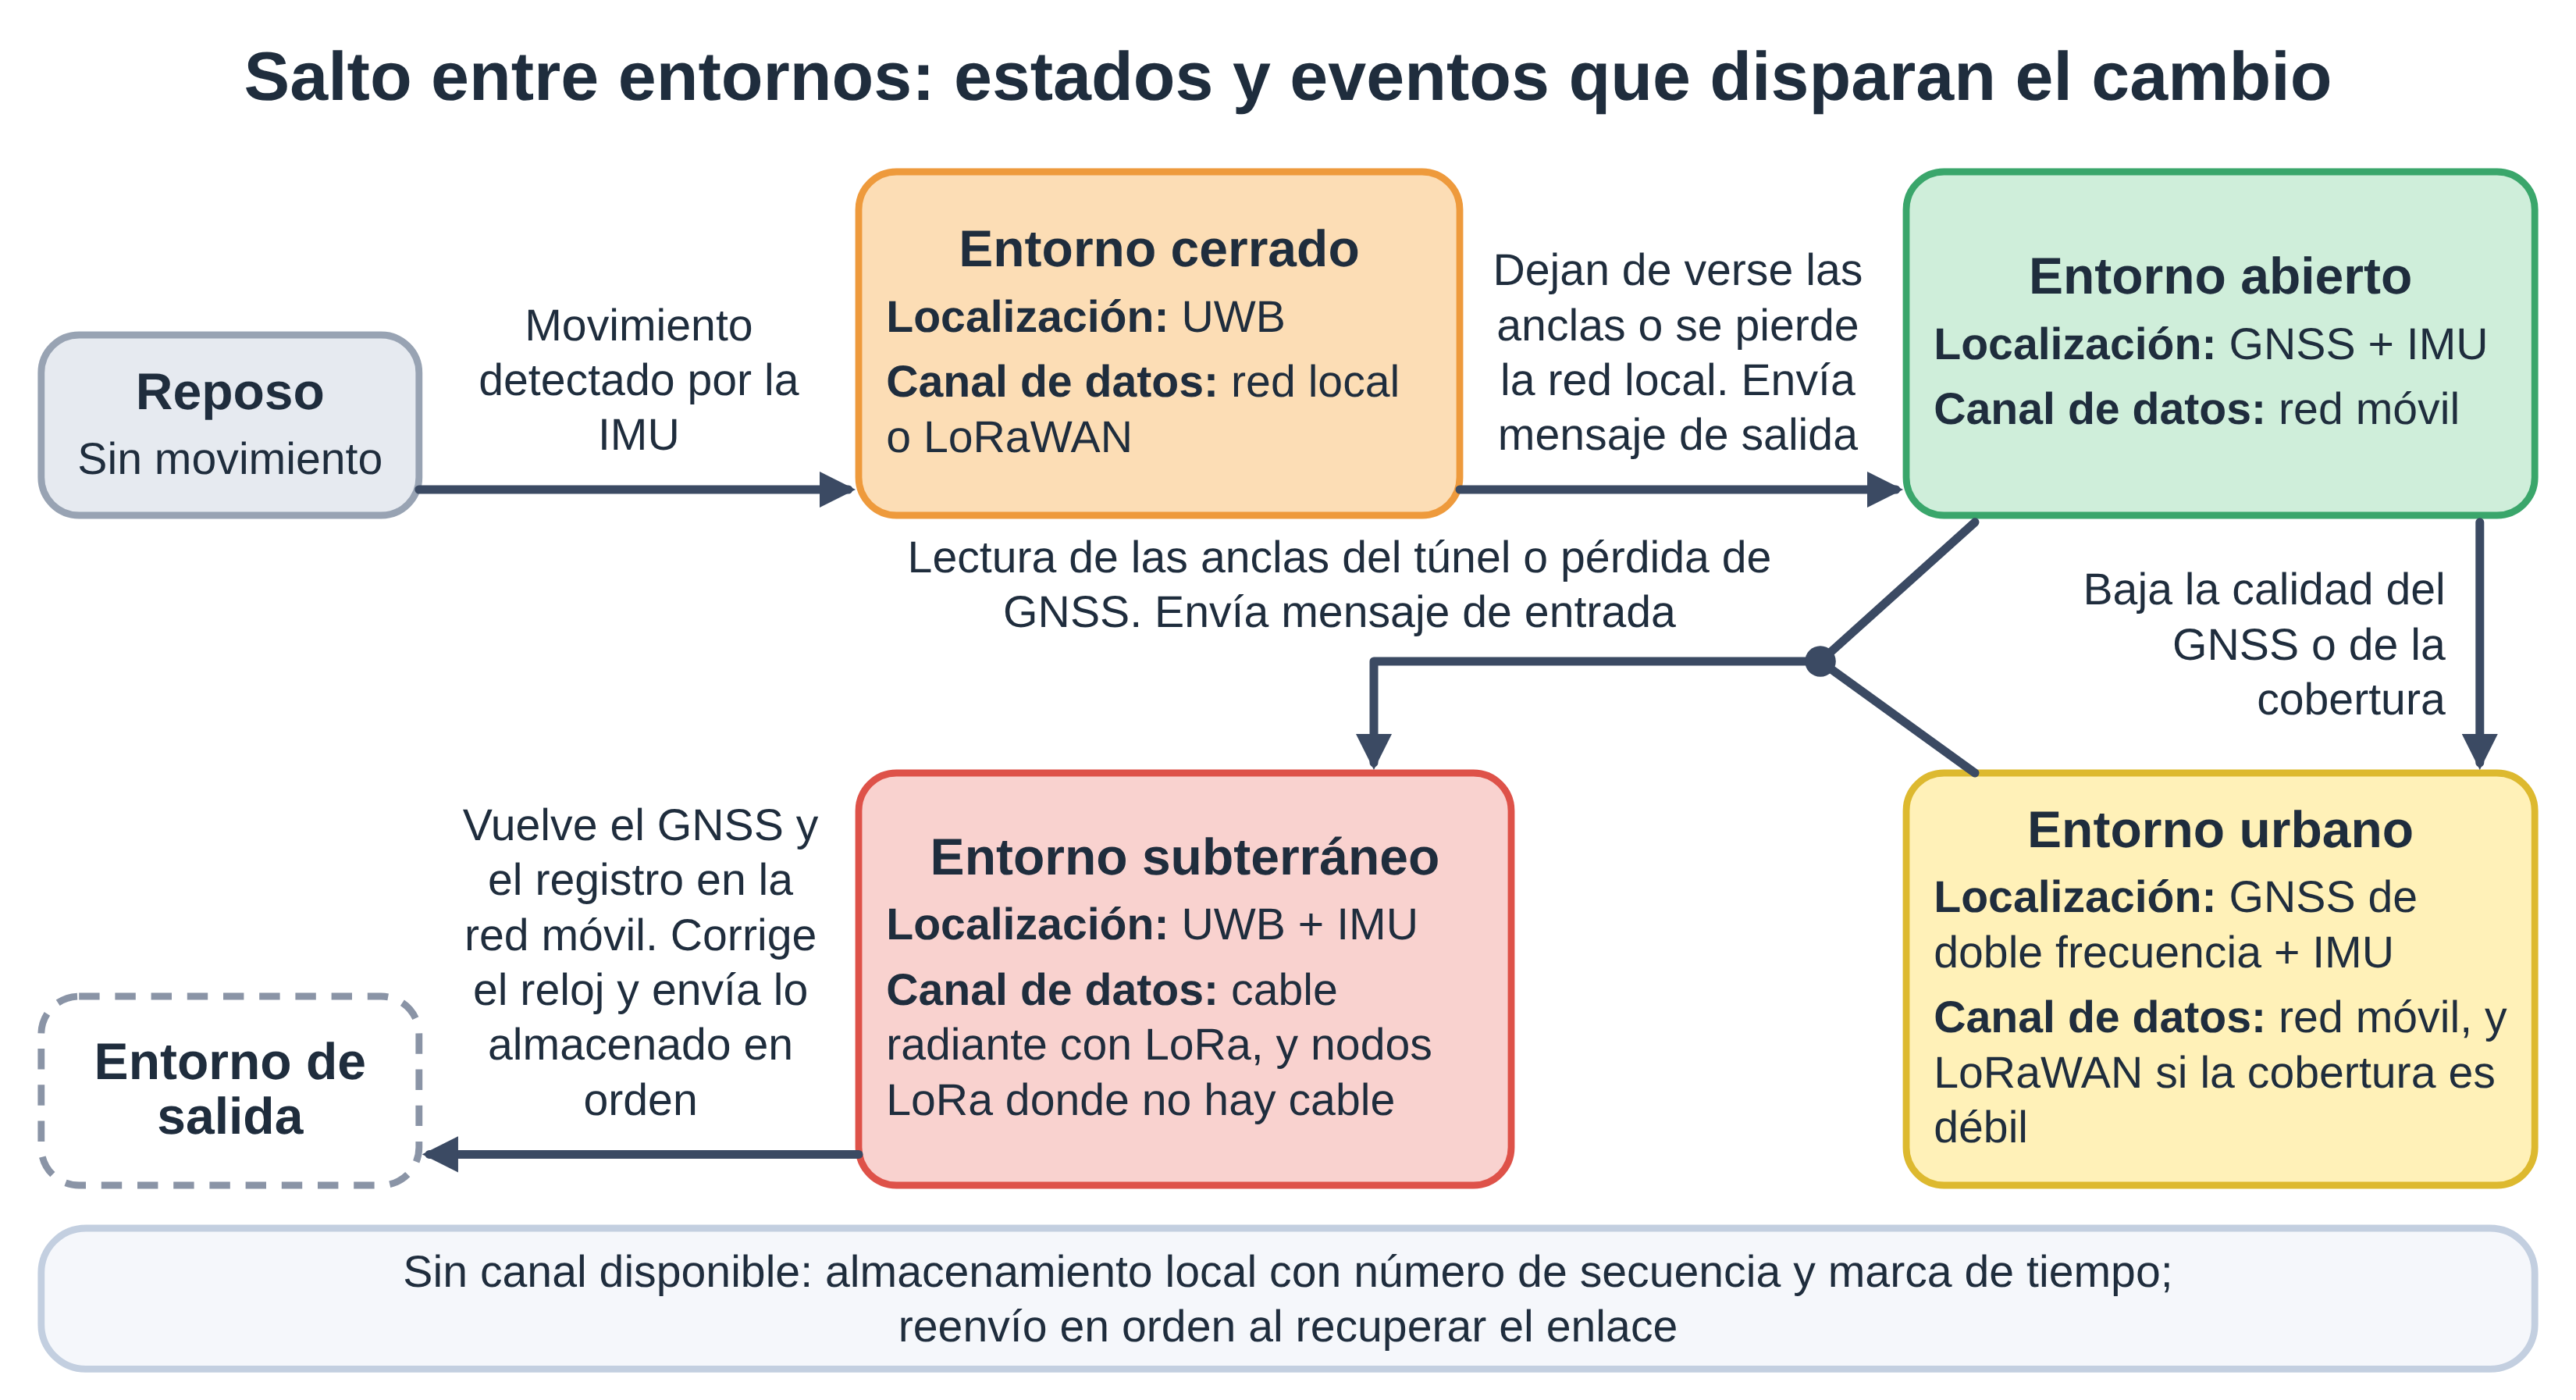
\includegraphics[width=\textwidth]{salto_entre_entornos_estados.png}
    \caption{Salto entre entornos: estados y eventos que disparan el cambio.}
    \label{fig:salto_estados}
\end{figure}

Así que se proponen cinco mecanismos complementarios:

\begin{itemize}
    \item \textbf{Máquina de estados con criterios de conmutación:} el firmware mantiene un estado de funcionamiento, que corresponde a uno de los cuatro entornos de la Sección~\ref{sec:apartado2}, es decir, abierto, urbano, cerrado o subterráneo, y evalúa continuamente unos indicadores. Se usa una máquina de estados porque el comportamiento depende del entorno actual y de pocos eventos, es fácil de comprobar y consume muy poco procesamiento en un microcontrolador. Para la localización, el GNSS se considera perdido cuando el número de satélites captados queda por debajo de un mínimo, o cuando el error estimado de la posición supera un límite, durante un tiempo determinado. Para las comunicaciones, el enlace del canal activo se considera perdido cuando falla el registro en la red o la potencia recibida cae bajo un umbral. Se exige que la condición se mantenga durante unos segundos porque una pérdida breve, como la de pasar bajo un puente, no justifica encender otro módem, que consume energía y tarda en registrarse. Además se usan umbrales distintos para entrar y para salir de un estado (histéresis), de modo que el dispositivo no cambie de tecnología una y otra vez cuando la señal está justo en el límite de ser utilizable.

    \item \textbf{Prioridad de fuentes de posición y fusión:} la posición se toma de la mejor fuente disponible según su precisión estimada. Primero el GNSS si es válido, porque no necesita infraestructura y su precisión basta cuando hay visión del cielo. Después el UWB si hay anclas a la vista, porque supera al GNSS en los entornos cerrados y subterráneos, donde las señales de satélite no llegan. Y en último lugar la estimación inercial, porque al integrar las aceleraciones el error crece con el tiempo (deriva) y solo es fiable en tramos cortos. Por esa misma razón la IMU no se usa sola, sino que se combina con la fuente activa mediante un algoritmo de fusión: la IMU estima el movimiento entre dos medidas y cada medida del GNSS o del UWB corrige el error que la IMU ha acumulado. Así, en cada cambio, la posición continúa desde la última estimada, sin reiniciarse ni dar saltos~\cite{ref14}.

    \item \textbf{Transiciones por eventos:} el cambio no espera a perder la cobertura porque la pérdida se detecta con retraso, ya que hay que esperar a que venzan tiempos de espera, y en ese intervalo se pierde información justo en la entrada de una zona ciega. Por eso se adelanta con eventos como el movimiento detectado por el acelerómetro o la lectura de las anclas UWB situadas en los límites de almacenes y túneles (en el caso en el que se esté utilizando la tecnología preferible UWB, en vez de otra de las mencionadas, como Wi-Fi RTT). Cada ancla tiene un identificador y una posición conocida, de modo que su lectura identifica el punto de paso y permite registrar el instante de entrada o salida, un dato que necesita el estudio de tiempos.

    \item \textbf{Selección del canal de datos con retroceso:} el dispositivo tiene definido para cada entorno un canal preferido para enviar sus mensajes a la plataforma y otros de respaldo, y los recorre por orden:
    \begin{itemize}
        \item \textbf{Entorno abierto:} red móvil como canal único porque tiene cobertura casi continua en carreteras y autopistas.

        \item \textbf{Entorno urbano:} red móvil como preferida, aunque su cobertura varía de una calle a otra, y LoRaWAN como respaldo en zonas de cobertura débil porque depende de puertas de enlace cuya cobertura no es universal.

        \item \textbf{Entorno cerrado:} red local del almacén como preferida porque ya existe y tiene mejor cobertura en interior, y LoRaWAN con puerta de enlace propia como alternativa.

        \item \textbf{Entorno subterráneo:} cable radiante como canal principal porque da cobertura continua en todo el túnel, y nodos LoRa donde no sea viable el cable.
    \end{itemize}

    Se intentan enviar los mensajes por el canal preferido y no se cambia al primer fallo, sino tras varios reintentos sin acuse, porque un fallo aislado no implica que el enlace se haya perdido. Si ningún canal responde, los mensajes pasan al almacenamiento local, que es el siguiente mecanismo. Los módems que no se usan se apagan para ahorrar energía, y el canal preferido se vuelve a probar periódicamente para regresar al más eficiente en cuanto se recupere.

    \item \textbf{Almacenamiento y reenvío con orden y deduplicación:} cuando ningún canal está disponible, el dispositivo guarda los mensajes en memoria no volátil, para no perderlos si el dispositivo se reinicia o la batería cae un momento. Cada mensaje lleva su número de secuencia, para ordenar los mensajes y detectar huecos, y la marca de tiempo del momento en que se midió la posición. La pone el dispositivo con su reloj interno y no la plataforma al recibir el mensaje, porque tras un periodo sin conexión los mensajes llegan mucho después de ocurrir y el estudio de tiempos necesita la hora del hecho. Ese reloj tiende a desajustarse con el tiempo, por lo que se corrige con la mejor referencia horaria disponible: la hora del GNSS cuando hay una posición válida y, en su defecto, la que proporciona la red al conectarse, ya sea la red móvil o una red local. Así, al entrar en una zona sin conexión, parte con la hora ajustada y el error acumulado durante el tramo es mínimo. Al recuperar la conexión los mensajes se envían por orden, priorizando los de entrada y salida frente a los puntos intermedios porque son los que alimentan el estudio de tiempos. Por LoRaWAN se escalonan para respetar el ciclo de trabajo y no saturar la puerta de enlace; por red móvil o por red local se agrupan en pocas conexiones para ahorrar energía. Cada mensaje se borra solo cuando se recibe su acuse para no perderlo si el reenvío falla. Este mecanismo no es nuevo: algunos dispositivos de seguimiento comerciales ya incorporan una caché de posiciones sin conexión~\cite{ref37}, y es el mismo principio de las redes tolerantes a retrasos y desconexiones, que almacenan los mensajes hasta que hay un enlace disponible para enviarlos~\cite{ref38}. Además, este mecanismo del dispositivo se complementa con el tratamiento que hace la plataforma al recibir los mensajes, ya que, gracias al formato común descrito en la Sección~\ref{sec:apartado5_1}, puede descartar duplicados, que pueden aparecer por reintentos o por varias puertas de enlace, y ordenar por la marca de tiempo del dispositivo y no por la hora de llegada, porque tras un reenvío en ráfaga los mensajes llegan juntos y puede que no en el orden real.
\end{itemize}

\subsection{Ejemplo de recorrido completo}
\label{sec:apartado5_3}

Para ver cómo trabajan juntos estos mecanismos, seguimos un paquete desde que sale de un almacén hasta que sale de un túnel, tal y como se resume en la Tabla~\ref{tab:ejemplo_recorrido}.

\begin{table}[H]
    \centering
    \footnotesize
    \renewcommand{\arraystretch}{1.15}
    \begin{tabular}{@{}L{2.2cm}L{3.7cm}L{4.7cm}L{3.7cm}@{}}
        \toprule
        \textbf{Situación} & \textbf{Evento que dispara el cambio} & \textbf{Qué hace el dispositivo} & \textbf{Motivo} \\
        \midrule
        \textbf{En el almacén} & Movimiento detectado por la IMU. & Sale de reposo y se localiza con las anclas UWB. Envía por la red local o por LoRaWAN. & Solo se activa cuando hay movimiento, para ahorrar batería. En el almacén el GNSS no funciona. \\
        \textbf{Sale del almacén} & Dejan de verse las anclas de localización o se pierde la red local del almacén. & Activa GNSS y red móvil. Envía un mensaje de salida y lo reenvía si no recibe acuse. & Las anclas marcan el instante de salida, que cierra la etapa de almacén y abre la de transporte. \\
        \textbf{Carretera} & Estado estable. & GNSS fusionado con IMU. Envía por red móvil. & El GNSS no necesita infraestructura y la IMU suaviza entre posiciones. La red móvil tiene cobertura casi continua. \\
        \textbf{Ciudad} & Entra en zona urbana y baja la calidad del GNSS o de la cobertura. & GNSS de doble frecuencia fusionado con IMU. Envía por red móvil y pasa a LoRaWAN si la cobertura es débil. & Los edificios bloquean o reflejan las señales y la cobertura varía de una calle a otra. \\
        \textbf{Llega al túnel} & Lectura de las anclas del túnel o pérdida de GNSS. & Pasa a UWB + IMU~\cite{ref23} y cambia al cable radiante con LoRa. Envía un mensaje de entrada y lo reenvía si no recibe acuse. & Sin satélites no hay GNSS. UWB e IMU mantienen la posición y el cable radiante da cobertura continua. \\
        \textbf{Dentro del túnel} & Sin acuse o sin enlace en algún tramo. & Envía por el cable radiante o, donde no hay cable, por nodos LoRa. Si el enlace se interrumpe, guarda los mensajes con secuencia y marca de tiempo. & Un corte puntual no debe suponer perder posiciones. \\
        \textbf{Salida del túnel} & Vuelve el GNSS y el registro en la red móvil. & Corrige el reloj, envía lo almacenado en orden, priorizando entradas y salidas, y pasa al estado del entorno en el que sale. & El GNSS y la red vuelven a estar disponibles para ajustar el reloj. Se envía por orden y se prioriza lo crítico para el estudio de tiempos. \\
        \bottomrule
    \end{tabular}
    \caption{Ejemplo de recorrido completo de un paquete y de los cambios de estado asociados.}
    \label{tab:ejemplo_recorrido}
\end{table}

\subsection{Entrega de los datos a la plataforma de gestión}
\label{sec:apartado5_4}

Superado el salto entre tecnologías, el recorrido es común. Sea cual sea el canal usado, los mensajes llegan a la plataforma por internet. La plataforma los valida, descarta duplicados y los guarda con el formato común descrito en la Sección~\ref{sec:apartado5_1}. La plataforma recibe y almacena los datos, y el personal de logística consulta la posición actual de los paquetes y su historial mediante la aplicación de gestión, que se comunica con la plataforma de dos maneras, porque responden a necesidades distintas. Por un lado, la plataforma ofrece una interfaz de servicio, como una interfaz de programación de aplicaciones (Application Programming Interface, API) de tipo REST (Representational State Transfer), que se consulta cuando el personal de logística pide el estado actual de un paquete o su historial, es decir, bajo demanda. Por otro lado, la plataforma envía avisos, por ejemplo por WebSocket o webhook, cuando ocurre un evento como la salida del almacén, para que el personal de logística lo conozca al instante sin tener que preguntar constantemente, lo que además ahorra tráfico de red. El tratamiento de estos datos y la información que muestra la aplicación se desarrollan en los apartados siguientes.

% =================================================================
% 6. INFRAESTRUCTURA EXTERNA
% =================================================================
\clearpage
\section{¿Qué antenas o elementos externos deberían ser desplegados?}
\label{sec:apartado6}

Una vez definidas las tecnologías de cada entorno (Sección~\ref{sec:apartado3}), los elementos que incorpora el paquete (Sección~\ref{sec:apartado4}) y la forma en que se comunican (Sección~\ref{sec:apartado5}), en este apartado se especifica la infraestructura que debe instalarse fuera del paquete para que esas tecnologías funcionen. El criterio seguido es desplegar infraestructura propia solo donde las redes públicas no llegan o no ofrecen la precisión necesaria, ya que, como recoge la Tabla~\ref{tab:criterios_entornos} de la Sección~\ref{sec:apartado2_3}, esta necesidad crece desde la carretera, donde generalmente es innecesaria, hasta el túnel, donde resulta imprescindible. Por ello, y dado que la empresa está dispuesta a desplegar los elementos necesarios, el esfuerzo se concentra en almacenes y túneles.

\subsection{Entorno abierto y urbano: aprovechamiento de la infraestructura existente}
\label{sec:apartado6_1}

En carreteras y zonas urbanas no se propone desplegar infraestructura propia de localización, puesto que la posición se obtiene directamente de las constelaciones GNSS y su precisión puede mejorarse mediante sistemas de aumentación basados en satélites (Satellite-Based Augmentation System, SBAS) como el European Geostationary Navigation Overlay Service (EGNOS), de uso gratuito en Europa y sin necesidad de instalar ningún elemento~\cite{ref8}. En cuanto a las comunicaciones, se utilizan las estaciones base de los operadores móviles, de modo que la empresa solo necesita contratar un servicio IoT con soporte LTE-M/NB-IoT (SIM o eSIM) y comprobar previamente la cobertura en las rutas habituales.

El respaldo LoRaWAN puede apoyarse en redes públicas existentes o en puertas de enlace propias instaladas en los centros logísticos y puntos de paso frecuentes, cuya cobertura alcanza también las zonas urbanas cercanas. Sin embargo, no se considera justificado desplegar una red LoRaWAN propia a lo largo de las carreteras, ya que su coste no compensa frente a la cobertura móvil disponible.

\subsection{Vehículo de transporte: pasarela embarcada (opcional)}
\label{sec:apartado6_2}

La Sección~\ref{sec:apartado4} señala que la recepción del dispositivo puede degradarse dentro de vehículos o embalajes metálicos, y es que una caja de carga metálica atenúa notablemente tanto la señal GNSS como la móvil. Para resolverlo se propone, como mejora opcional, instalar en cada vehículo una pasarela embarcada formada por una puerta de enlace LoRaWAN en el interior de la zona de carga y antenas externas GNSS y móvil en el techo, alimentada por la batería del vehículo. De este modo, los paquetes se comunican con la pasarela a corta distancia y con poca potencia, mientras que esta reenvía los datos por la red móvil.

Esta solución reduce el consumo de los dispositivos, hace las comunicaciones más robustas y permite, además, saber en qué vehículo viaja cada paquete. Aun así, no sustituye a los módulos del propio paquete, que siguen siendo necesarios cuando no viaja en un vehículo equipado, ni resuelve el túnel, donde la pasarela también pierde la red móvil.

\subsection{Entorno cerrado: almacenes y centros logísticos}
\label{sec:apartado6_3}

La Figura~\ref{fig:infraestructura_almacen} muestra la infraestructura propia que se despliega en el entorno cerrado.

\begin{figure}[H]
    \centering
    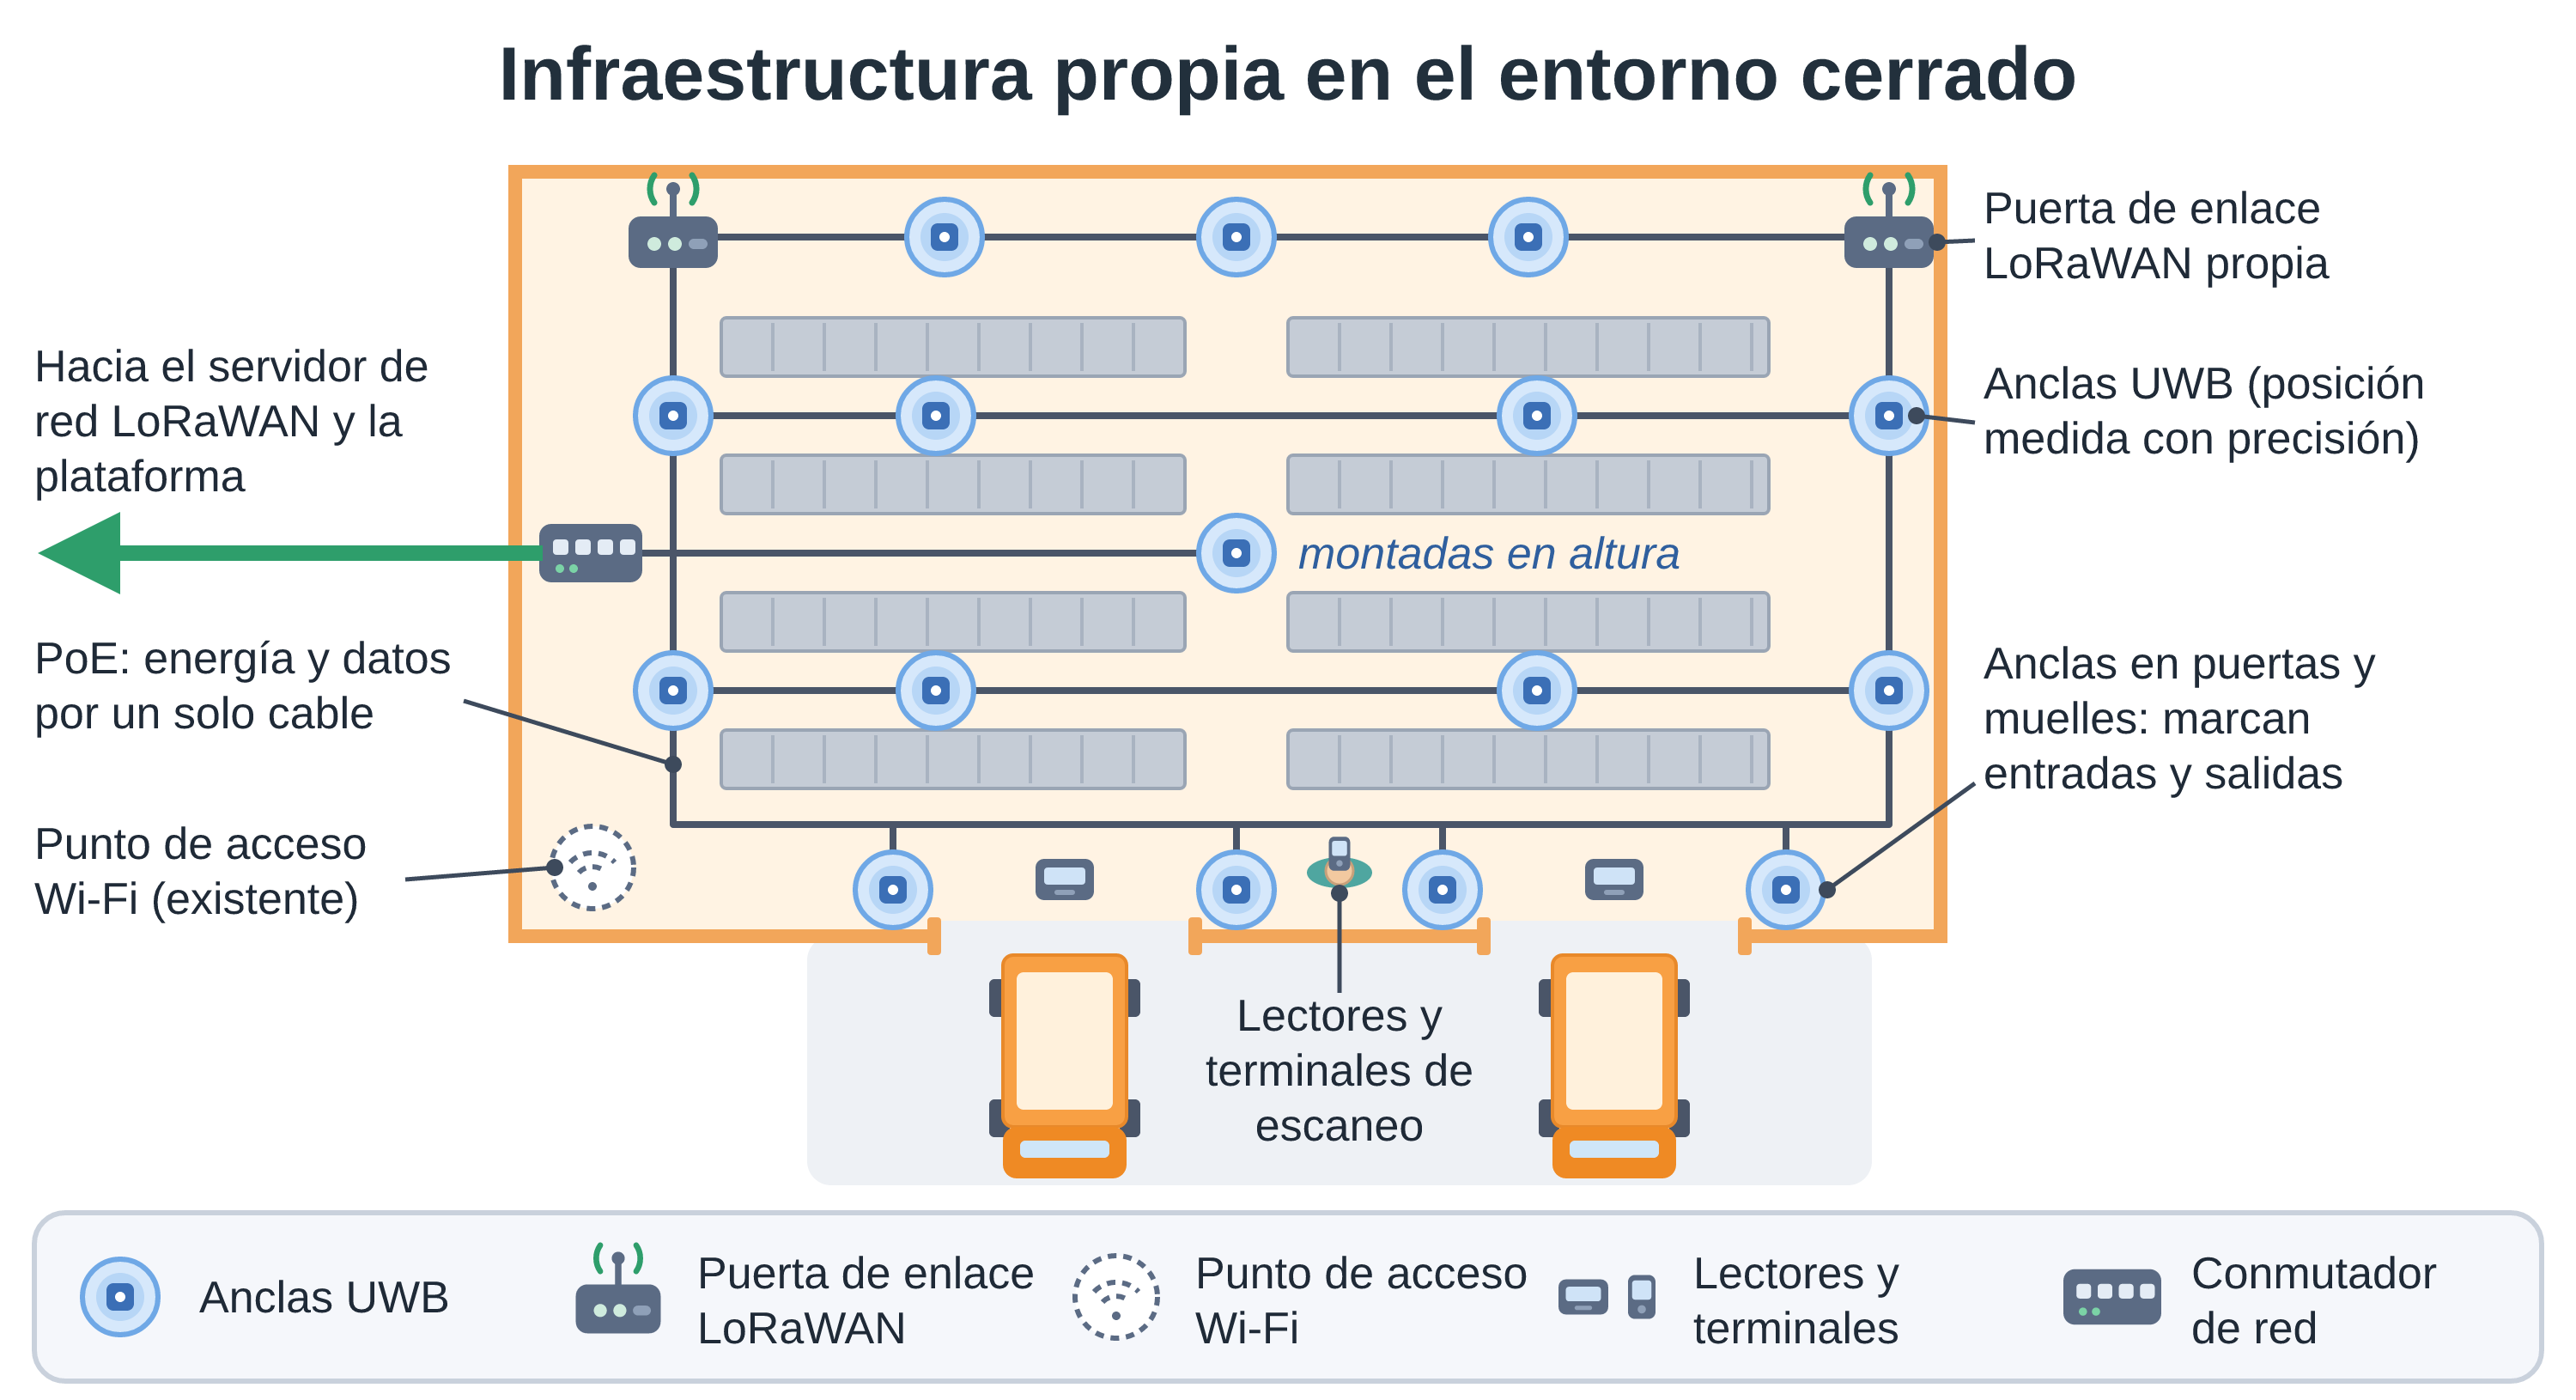
\includegraphics[width=\textwidth]{infraestructura_entorno_cerrado.png}
    \caption{Infraestructura propia en el entorno cerrado.}
    \label{fig:infraestructura_almacen}
\end{figure}

\textbf{Anclas UWB.} Son el elemento principal de localización interior y se instalan en posiciones fijas cuyas coordenadas deben medirse con precisión, ya que cualquier error en la posición de un ancla se traslada directamente a la posición calculada del paquete. Conviene montarlas en altura, por encima de las estanterías, para mantener visión directa con los paquetes, y distribuirlas de forma que desde cualquier punto se vean al menos tres anclas para localizar en el plano, o cuatro si se necesita la altura. En las zonas con estanterías metálicas, donde se producen más reflexiones~\cite{ref6}, la densidad de anclas debe ser mayor.

Además, deben colocarse anclas en las puertas y muelles de carga, cuya lectura permite registrar los eventos de entrada y salida descritos en la Sección~\ref{sec:apartado5_2}. Todas ellas se alimentan y conectan mediante Power over Ethernet (PoE)~\cite{ref39}, que con un único cable proporciona tanto la energía como la conexión para su configuración y supervisión.

Si el número de paquetes simultáneos es elevado, la medida por two-way ranging (Sección~\ref{sec:apartado5_1}) escala peor porque cada medida ocupa el canal radio, por lo que puede emplearse Time Difference of Arrival (TDoA), aunque esta técnica exige sincronizar las anclas entre sí, por cable o por radio. En cualquier caso, los equipos UWB deben cumplir la norma armonizada ETSI EN 302 065 del European Telecommunications Standards Institute (ETSI)~\cite{ref40}.

\textbf{Puertas de enlace LoRaWAN propias.} Se instalan una o varias según el tamaño de la nave, con la antena en una posición elevada y alejada de estanterías y estructuras metálicas, ya que en naves grandes o muy metálicas una sola puerta de enlace dejaría zonas sin cobertura. Se conectan por Ethernet al servidor de red LoRaWAN y su cobertura puede extenderse también a la playa de maniobras exterior. Los equipos de 868~MHz deben cumplir la norma ETSI EN 300 220 y las limitaciones de ciclo de trabajo de la banda~\cite{ref26,ref28}.

\textbf{Puntos de acceso Wi-Fi.} Se reutiliza la red existente para el transporte de datos, aunque, si se optara por la localización mediante Wi-Fi RTT o Bluetooth Channel Sounding (Sección~\ref{sec:apartado3_4}), los puntos de acceso o balizas tendrían que admitir expresamente esas funciones~\cite{ref18,ref19}.

\textbf{Terminales de escaneo.} Como el registro de la recogida y la entrega se realiza escaneando el identificador del paquete (Sección~\ref{sec:apartado4_2}), se necesitan lectores en los muelles y terminales portátiles para los repartidores, conectados a la red local o a la red móvil.

\subsection{Entorno subterráneo: túneles}
\label{sec:apartado6_4}

El túnel es el entorno que más infraestructura requiere, ya que tanto la localización como la comunicación con el exterior dependen por completo de elementos propios.

\textbf{Cable radiante.} Constituye la columna vertebral de las comunicaciones (Secciones~\ref{sec:apartado3_5} y~\ref{sec:apartado5_1}) y se tiende a lo largo de todo el túnel, fijado al techo o a la parte alta de la pared mediante soportes que lo separan de la superficie, puesto que la proximidad a la pared degrada su acoplamiento con los dispositivos. Debe elegirse un modelo dimensionado para la banda de 868~MHz~\cite{ref20,ref31}, cuya atenuación a lo largo del cable y cuya pérdida de acoplamiento determinan el balance del enlace. Como la atenuación crece con la frecuencia y la longitud, es necesario intercalar amplificadores de línea bidireccionales a intervalos que dependen del modelo de cable y terminar el tendido con una carga adaptada. Además, al tratarse de un espacio confinado, el cable y los equipos deben tener cubierta resistente al fuego y libre de halógenos.

Si el túnel ya dispone de un cable radiante para radiocomunicaciones de emergencia, podría estudiarse con su titular la posibilidad de compartirlo mediante equipos multibanda, lo que reduciría el coste del despliegue.

\textbf{Puerta de enlace de cabecera.} En la boca del túnel se instala una puerta de enlace LoRaWAN conectada al cable radiante mediante un acoplador, que lleva los datos al exterior por fibra o Ethernet o, si en la boca no hay red cableada, mediante un router móvil con antena exterior. En túneles largos se recomienda instalar una en cada boca, de modo que haya redundancia y ningún tramo quede aislado si el cable se corta.

\textbf{Nodos repetidores LoRa.} En los tramos donde no sea viable tender cable, como curvas cerradas, ramales o zonas provisionales, se instalan nodos LoRa que pueden encadenarse formando una malla lineal~\cite{ref21,ref33}. No obstante, cada salto añade retardo y consume ciclo de trabajo, por lo que conviene limitar su número. Se alimentan de la instalación eléctrica del túnel o, si no existe, con baterías sujetas a un plan de mantenimiento.

\textbf{Anclas UWB.} Se distribuyen a lo largo del túnel para la localización asistida por inercia propuesta en la Sección~\ref{sec:apartado3_5}~\cite{ref23}. Aunque la forma larga y estrecha del túnel no favorece la trilateración en el plano, esta tampoco es necesaria, ya que lo relevante es la posición a lo largo del eje del túnel. Por ello basta con colocar las anclas alternadas en las paredes, con una separación fijada mediante medidas de campo que garantice que el dispositivo vea siempre al menos dos. Las anclas de cada boca actúan como puerta y permiten registrar los eventos de entrada y salida del túnel. Todas se alimentan de la instalación eléctrica del túnel o mediante PoE desde conmutadores conectados a una fibra tendida junto al cable radiante.

\textbf{Referencia temporal.} La puerta de enlace también puede proporcionar la hora de red a los dispositivos mediante el comando DeviceTimeReq de LoRaWAN~\cite{ref35}, de manera que las marcas de tiempo registradas dentro del túnel no dependan solo de la deriva del reloj interno, lo que complementa la corrección por GNSS a la salida descrita en la Sección~\ref{sec:apartado5_2}.

\textbf{Alternativa descartada: repetidores GNSS.} Un repetidor GNSS capta la señal de los satélites en el exterior y la retransmite dentro del túnel, pero se descarta porque requiere autorización administrativa~\cite{ref41}, puede interferir con receptores cercanos y, sobre todo, hace que todos los dispositivos en su zona de cobertura calculen la posición de la antena exterior y no la suya propia, por lo que no sirve para localizar el paquete dentro del túnel.

\subsection{Resumen de elementos a desplegar}
\label{sec:apartado6_5}

La Tabla~\ref{tab:elementos_desplegar} resume los elementos externos que deben desplegarse en cada entorno.

\begin{table}[H]
    \centering
    \footnotesize
    \renewcommand{\arraystretch}{1.15}
    \begin{tabular}{@{}L{2.9cm}L{4.5cm}L{4.2cm}L{3.1cm}@{}}
        \toprule
        \textbf{Entorno} & \textbf{Elemento externo} & \textbf{Función} & \textbf{Alimentación y conexión} \\
        \midrule
        Carretera y urbano & Ninguno propio: satélites GNSS, EGNOS y estaciones base del operador & Posición y transporte de datos & Contrato de servicio IoT \\
        Carretera y urbano (opcional) & Puertas de enlace LoRaWAN en centros logísticos & Respaldo de comunicaciones & Red eléctrica y Ethernet \\
        Vehículo (opcional) & Pasarela embarcada con antenas GNSS y móvil en el techo & Evitar el apantallamiento de la caja e identificar el vehículo & Batería del vehículo y red móvil \\
        Almacén & Anclas UWB, incluidas puertas y muelles & Localización interior y eventos de entrada y salida & PoE \\
        Almacén & Puertas de enlace LoRaWAN & Transmisión de bajo consumo & PoE o red eléctrica y Ethernet \\
        Almacén & Puntos de acceso Wi-Fi (existentes) & Transporte de datos y, si se admite, Wi-Fi RTT & Red local \\
        Recogida y entrega & Lectores en muelles y terminales del repartidor & Registro de recogida y entrega & Red local o red móvil \\
        Túnel & Cable radiante con amplificadores de línea y carga terminal & Columna vertebral de comunicaciones & Alimentación de los amplificadores \\
        Túnel & Puerta de enlace LoRaWAN de cabecera, en una o ambas bocas & Llevar los datos al exterior & Fibra, Ethernet o router móvil \\
        Túnel & Nodos repetidores LoRa & Cubrir tramos sin cable & Instalación del túnel o baterías \\
        Túnel & Anclas UWB a lo largo del túnel y en las bocas & Posición en el túnel y eventos & Instalación del túnel, PoE o baterías \\
        \bottomrule
    \end{tabular}
    \caption{Resumen de los elementos externos que deben desplegarse en cada entorno.}
    \label{tab:elementos_desplegar}
\end{table}

\subsection{Consideraciones de despliegue}
\label{sec:apartado6_6}

\textbf{Estudio previo de campo.} El número y la posición de anclas, puertas de enlace y amplificadores no puede fijarse de antemano, sino que debe determinarse mediante medidas en cada almacén y túnel con paquetes cargados en condiciones reales.

\textbf{Supervisión de la infraestructura.} Las anclas y puertas de enlace deben enviar periódicamente un mensaje de estado a la plataforma, de forma que un fallo de la infraestructura se detecte como tal y no se confunda con una incidencia del paquete. Esta información puede alimentar, además, las alertas de la aplicación de gestión (Sección~\ref{sec:apartado8}).

\textbf{Protección y mantenimiento.} Los equipos deben instalarse fuera del alcance de carretillas y vehículos y protegidos frente a impactos y manipulaciones, ya que un ancla desplazada falsea las posiciones calculadas. En los túneles, por su parte, el mantenimiento requiere coordinarse con el titular de la infraestructura para los permisos de acceso y la sustitución de baterías.

\textbf{Normativa radioeléctrica.} Todos los equipos deben cumplir las normas armonizadas de su banda, es decir, ETSI EN 302 065 para UWB y ETSI EN 300 220 para 868~MHz, incluidas las limitaciones de ciclo de trabajo~\cite{ref26,ref40,ref28}.

En conclusión, la infraestructura propia se concentra en almacenes y túneles, mientras que en carretera y ciudad basta con las redes públicas existentes, con la pasarela embarcada como mejora opcional. En los túneles, la combinación de cable radiante, puertas de enlace de cabecera y anclas UWB es la que hace posible el seguimiento en un entorno que, inicialmente, no dispone de ningún tipo de comunicación.

% =================================================================
% 7. PLATAFORMA DE GESTIÓN
% =================================================================
\clearpage
\section{¿Qué elementos debería tener la plataforma para tratar con los datos?}
\label{sec:apartado7}

La plataforma es el destino de los cuatro canales de la Sección~\ref{sec:apartado5_1} y fuente de la aplicación de la Sección~\ref{sec:apartado8}. No basta con un panel: se propone organizarla en seis bloques que siguen el recorrido del dato (ingesta, procesamiento, almacenamiento y exposición) y añaden la gestión de dispositivos e infraestructura y la seguridad. Esta separación es coherente con oneM2M, que sitúa una capa de servicios comunes con funciones de gestión de datos, dispositivos, seguridad y comunicación~\cite{ref42}, y con la división de LoRaWAN entre servidor de red y servidor de aplicación~\cite{ref24}. La estructura propuesta se resume en la Figura~\ref{fig:plataforma}.

\begin{figure}[H]
    \centering
    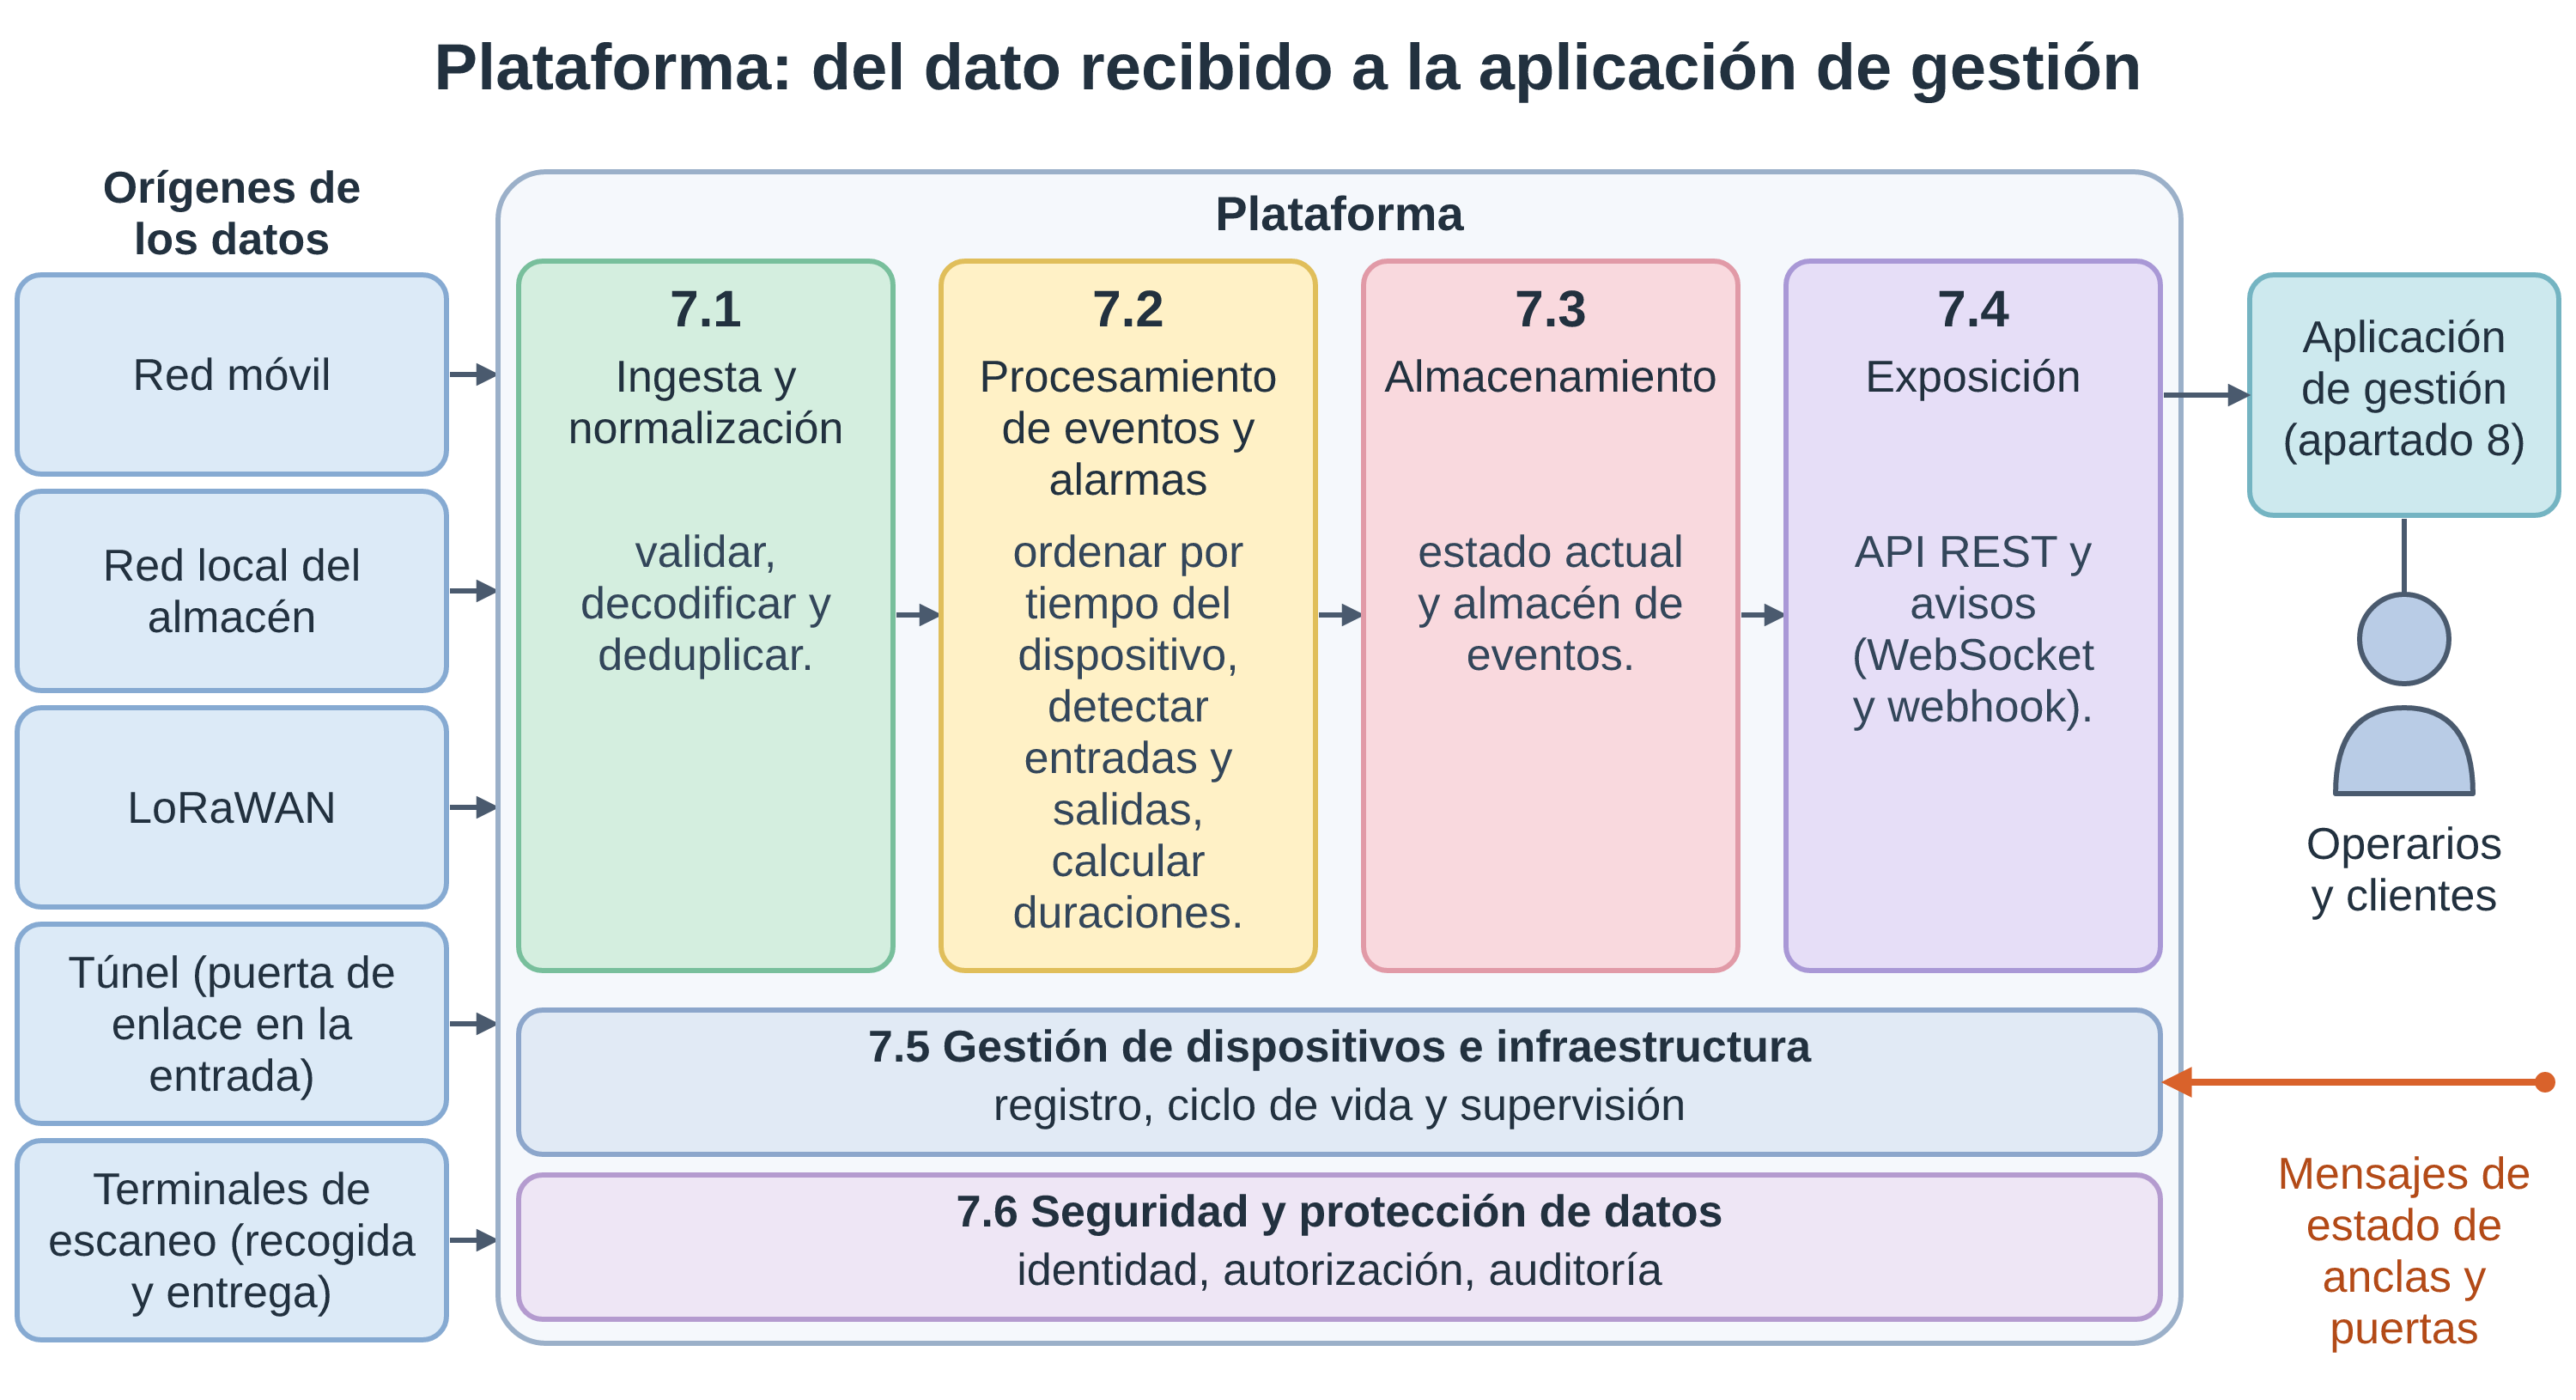
\includegraphics[width=\textwidth]{figura_plataforma.png}
    \caption{Plataforma: del dato recibido a la aplicación de gestión.}
    \label{fig:plataforma}
\end{figure}

\subsection{Ingesta multicanal y normalización}
\label{sec:apartado7_1}

La ingesta es una capa con un punto de entrada por canal, que acepta MQTT~\cite{ref30} sobre TLS, CoAP~\cite{ref29} sobre DTLS, un \emph{endpoint} Hypertext Transfer Protocol Secure (HTTPS) de entrada para los webhooks del servidor de aplicación y para los escaneos~\cite{ref43}. En LoRaWAN la plataforma debe actuar como servidor de aplicación o conectarse a uno: el servidor de red enruta y deduplica, mientras que el descifrado y la decodificación del payload corresponden al servidor de aplicación~\cite{ref24,ref43}. Sin esa pieza no se interpreta el formato común de la Sección~\ref{sec:apartado5_1}.

Un normalizador convierte el mensaje binario en un registro canónico con los campos de la Sección~\ref{sec:apartado5_1} y añade canal, puerta de enlace y hora de llegada. La validación comprueba que el identificador existe, que la secuencia y la marca de tiempo son coherentes y los valores están en rango. Los mensajes que no pasan se conservan en cuarentena.

Se deduplica por (paquete, secuencia). El servidor de red elimina copias LoRaWAN~\cite{ref24} y CoAP detecta duplicados por \emph{Message ID}~\cite{ref29}, pero un registro puede llegar por varios canales o repetirse. Se propone una clave única en el almacén. Para los mensajes críticos de la Sección~\ref{sec:apartado5_1}, la ingesta debe distinguir el acuse de red (en LoRaWAN lo genera el servidor de red~\cite{ref24,ref35}) del acuse de persistencia, y no marcar el evento como recibido hasta que esté escrito.

\subsection{Procesamiento de eventos y alarmas}
\label{sec:apartado7_2}

El procesamiento trabaja con el tiempo del dispositivo, no con el de llegada, como exige la Sección~\ref{sec:apartado5_2}. Ordena cada paquete por marca de tiempo y secuencia y aplica una ventana de tolerancia para lotes tardíos tras un túnel o un corte; se priorizan las entradas y salidas frente a las posiciones intermedias. Esa ventana es una decisión de diseño.

El procesador convierte las posiciones en estados y eventos: recogida, salida del almacén, entrada y salida del túnel, llegada y entrega. Cruza cada lectura con el registro de anclas y puertas, con su identificador y posición conocida (Secciones~\ref{sec:apartado5_2} y~\ref{sec:apartado6_3}), y con los escaneos de la Sección~\ref{sec:apartado4_2}. No deduce una entrega porque el paquete se detenga. Con esos eventos calcula la duración total y las duraciones por etapa o entorno, que necesita la Sección~\ref{sec:apartado8_2}. El estado del envío se propone derivarlo de esos eventos: recogido, en tránsito, en túnel, entregado o incidencia.

Mantiene el estado actual: última posición, última actualización, tecnología activa, batería, precisión y huecos de secuencia. Se propone un motor de reglas que evalúe condiciones y mantenga alarmas con estado (activa, reconocida, cerrada) para batería baja, falta de actualizaciones, retraso o incidencia. ThingsBoard incorpora uno para filtrar y transformar mensajes~\cite{ref44}.

Para distinguir ``sin datos por el túnel'' de ``dispositivo averiado'' se combina el último entorno conocido con los latidos de anclas y puertas de la Sección~\ref{sec:apartado6_6}. Si la infraestructura del túnel sigue reportando y el paquete no, se señala el dispositivo. Si también callan las anclas y la puerta, se señala la infraestructura.

\subsection{Almacenamiento}
\label{sec:apartado7_3}

Se propone separar dos almacenes. El primero guarda el estado actual de cada envío y de cada dispositivo: última posición, último evento, batería, precisión, tecnología y estado de comunicación; lo consulta la API y alimenta la última posición confirmada del túnel (Sección~\ref{sec:apartado8_3}). El segundo es un almacén de eventos y series temporales, solo de adición, con todas las posiciones y eventos, sus marcas de tiempo y el canal por el que llegaron. Permite reconstruir el recorrido, recalcular duraciones y auditar una incidencia. El registro de envíos guarda origen, destino y dispositivo.

El almacén de eventos conserva el payload original y el registro decodificado, para poder reprocesar si cambia el decodificador. La clave (paquete, secuencia) impide duplicados y las consultas se indexan por paquete y por intervalo temporal. Se propone una retención distinta para el dato bruto y para el histórico agregado, y aplicar desde el diseño la minimización y la limitación del plazo del Reglamento General de Protección de Datos (RGPD)~\cite{ref45}.

\subsection{Exposición de datos y avisos}
\label{sec:apartado7_4}

La plataforma debe ofrecer una API REST para consultas bajo demanda y un canal de notificaciones para los avisos, como anticipa la Sección~\ref{sec:apartado5_4}. La API expone el envío (identificador, origen, destino y estado), la última posición con su hora y precisión, el recorrido, las horas de recogida, actualización, entrada y salida de cada entorno y entrega, la tecnología activa, los huecos de secuencia (para estimar los mensajes pendientes), la batería y el historial de eventos y alertas. Son los datos que necesita la Sección~\ref{sec:apartado8_2}.

Las notificaciones se envían por WebSocket cuando la aplicación mantiene una conexión abierta, y por webhook cuando el destinatario es otro sistema. WebSocket proporciona un canal bidireccional sobre una sola conexión TCP~\cite{ref46}, y el webhook es una petición HTTP(S) a un extremo del receptor; The Things Stack la intenta una sola vez por defecto y los reintentos son una función opcional~\cite{ref47}, por lo que se propone que la plataforma los incorpore para no perder avisos si el receptor está caído.

La API debe estar versionada y con inventario de endpoints; un endpoint antiguo o de depuración es un riesgo recogido por Open Worldwide Application Security Project (OWASP)~\cite{ref48}. La autorización se comprueba por objeto, no solo por rol: un usuario no debe consultar un envío ajeno cambiando el identificador~\cite{ref48}.

\subsection{Gestión de dispositivos e infraestructura}
\label{sec:apartado7_5}

La plataforma necesita un registro de lo que produce datos: dispositivos de paquete, anclas UWB y puertas de enlace LoRaWAN. Para cada dispositivo guarda un identificador único, el tipo, el envío asociado, el firmware, las credenciales, la configuración y el estado. Para cada ancla, además, su posición conocida y el punto de paso que representa (puerta, muelle o boca de túnel), porque sin esa correspondencia no se interpretan entradas y salidas (Secciones~\ref{sec:apartado5_2}, \ref{sec:apartado6_3} y~\ref{sec:apartado6_4}).

Cubre el ciclo de vida: alta, asignación a un envío, sustitución, baja y rotación de claves. NISTIR 8259A incluye la identificación única y el control de acceso lógico a las interfaces de un dispositivo IoT~\cite{ref49}, y oneM2M sitúa la gestión de dispositivos como función común del servicio~\cite{ref42}.

La supervisión usa los mensajes periódicos de estado de la Sección~\ref{sec:apartado6_6}. La plataforma guarda la última vez visto y la batería de cada elemento, y compara el silencio con el intervalo esperado. Así separa una incidencia de infraestructura de una del paquete y evita que un fallo de la puerta del túnel se lea como avería del dispositivo.

\subsection{Seguridad y protección de datos}
\label{sec:apartado7_6}

La seguridad de la plataforma no queda cubierta por el cifrado de transporte de la Sección~\ref{sec:apartado5_1}. Se proponen cuatro controles. El primero es la identidad de los dispositivos: credenciales propias y revocables, y autenticación de dispositivo y de usuario; NISTIR 8259A recoge la identificación única y el acceso lógico restringido~\cite{ref49}. En LoRaWAN, el servidor de unión reparte la NwkSKey al servidor de red y la AppSKey al servidor de aplicación~\cite{ref24,ref35}; la plataforma debe custodiar solo la que necesita para descifrar.

El segundo es la identidad de las personas: autenticación, segundo factor para administradores y autorización por rol y por objeto. OWASP API Security Top 10 (2023) sitúa la autorización a nivel de objeto y la autenticación rota entre los riesgos principales de una API~\cite{ref48}. El tercero es la protección de la API: mitigación del consumo desmedido de recursos, gestión de inventario de versiones~\cite{ref48} y la validación estricta de datos entrantes. El cuarto es la auditoría: un registro inmutable de accesos y cambios, con retención definida; NISTIR 8259A incluye que el dispositivo pueda informar de su estado de ciberseguridad a entidades autorizadas~\cite{ref49}, información que la plataforma debería registrar.

El RGPD es aplicable si los datos permiten identificar a una persona. El artículo 4 considera datos personales los datos de localización cuando hacen identificable al interesado~\cite{ref45}; la posición de un paquete, por sí sola, no identifica a nadie, pero si se asocia al repartidor que lo escanea o al terminal que lo acompaña, sí puede hacerlo.

En ese caso la plataforma debe separar la identidad del envío de la del empleado, limitar quién puede cruzar ambos datos y aplicar minimización y limitación del plazo de conservación (artículo 5)~\cite{ref45}. Si no puede establecerse ese vínculo, la aplicación del RGPD no puede afirmarse sin más; es una duda que debe resolver el responsable del tratamiento.

\subsection{Síntesis}
\label{sec:apartado7_7}

La Tabla~\ref{tab:sintesis_plataforma} resume los elementos y su trazabilidad a los requisitos del resto del trabajo. No es una lista de productos, sino el conjunto mínimo para que los datos de las Secciones~\ref{sec:apartado3} a~\ref{sec:apartado6} lleguen a la aplicación de la Sección~\ref{sec:apartado8} sin pérdidas ni ambigüedades.

\begin{table}[H]
    \centering
    \footnotesize
    \renewcommand{\arraystretch}{1.15}
    \begin{tabular}{@{}L{4.9cm}L{6.7cm}L{3.5cm}@{}}
        \toprule
        \textbf{Elemento de la plataforma} & \textbf{Función} & \textbf{Requisito del que procede} \\
        \midrule
        Capa de ingesta multicanal & Termina MQTT, CoAP y HTTPS; autentica y normaliza & \ref{sec:apartado5_1} \\
        Decodificador y registro canónico & Interpreta el formato común y valida los campos & \ref{sec:apartado5_1}, \ref{sec:apartado4_2} \\
        Deduplicador idempotente & Una sola unidad por (paquete, secuencia) & \ref{sec:apartado5_2}, \ref{sec:apartado5_4} \\
        Procesador de eventos & Ordena por tiempo del dispositivo, detecta entradas y salidas y calcula duraciones & \ref{sec:apartado5_2}, \ref{sec:apartado5_4}, \ref{sec:apartado4_2}, \ref{sec:apartado6_3} \\
        Motor de reglas y alarmas & Batería, silencio, retraso e incidencia; distingue túnel de avería & \ref{sec:apartado8_2}, \ref{sec:apartado6_6}, \ref{sec:apartado8_3} \\
        Estado actual & Última posición, batería, tecnología y huecos de secuencia & \ref{sec:apartado5_4}, \ref{sec:apartado8_2}, \ref{sec:apartado8_3} \\
        Almacén de eventos y series temporales & Histórico, recorrido, auditoría y reproceso & \ref{sec:apartado5_2}, \ref{sec:apartado8_2} \\
        API REST y avisos WebSocket/webhook & Consulta bajo demanda y notificación de eventos & \ref{sec:apartado5_4}, \ref{sec:apartado8_2} \\
        Registro de dispositivos, anclas y puertas & Identidad, posición conocida, ciclo de vida y estado & \ref{sec:apartado5_2}, \ref{sec:apartado6_3}, \ref{sec:apartado6_4}, \ref{sec:apartado6_6} \\
        Seguridad y auditoría & Identidad, autorización, claves, trazas y protección de datos & \ref{sec:apartado5_1}; RGPD~\cite{ref45} \\
        \bottomrule
    \end{tabular}
    \caption{Síntesis de los elementos de la plataforma y su trazabilidad a los requisitos del trabajo.}
    \label{tab:sintesis_plataforma}
\end{table}

% =================================================================
% 8. APLICACIÓN DE GESTIÓN
% =================================================================
\clearpage
\section{¿Qué contenido se debería poder visualizar en la aplicación de gestión?}
\label{sec:apartado8}

\subsection{Objetivo de la aplicación}
\label{sec:apartado8_1}

La aplicación de gestión debe ser la interfaz mediante la cual el personal de logística puede consultar la información recogida por los dispositivos instalados en los paquetes. Su objetivo principal sería permitir el seguimiento de la mercancía durante todo el trayecto, desde la recogida, hasta la entrega al cliente.

\subsection{Información que debe mostrar}
\label{sec:apartado8_2}

La aplicación deberá contemplar las limitaciones y comunicación de cada entorno. La información que debería mostrar se resume en la Tabla~\ref{tab:informacion_app}.

\begin{table}[H]
    \centering
    \footnotesize
    \renewcommand{\arraystretch}{1.15}
    \begin{tabular}{@{}L{3.5cm}L{6.8cm}L{4.4cm}@{}}
        \toprule
        \textbf{Bloque} & \textbf{Información que mostraría} & \textbf{Para qué sirve} \\
        \midrule
        Identificación del paquete & ID único, origen, destino y estado del envío & Identificar cada paquete \\
        Localización & Posición actual o última conocida, mapa y recorrido & Seguir el paquete durante su transporte \\
        Tiempos & Hora de recogida, última actualización, entrada y salida de cada entorno y entrega & Calcular la duración total y de cada etapa \\
        Estado de las comunicaciones & Tecnología activa, conexión disponible y mensajes pendientes de enviar & Detectar pérdidas de cobertura y retrasos en la actualización \\
        Estado del dispositivo & Batería, precisión estimada de la posición & Comprobar que el seguimiento funciona correctamente \\
        Historial de eventos & Recogida, salida del almacén, entrada y salida del túnel, llegada al destino y entrega & Reconstruir el recorrido y verificar los tiempos registrados \\
        Alertas & Batería baja, falta de actualizaciones, retrasos o incidencias & Facilitar la supervisión y la intervención cuando sea necesaria \\
        \bottomrule
    \end{tabular}
    \caption{Información que debe mostrar la aplicación de gestión.}
    \label{tab:informacion_app}
\end{table}

\subsection{Comportamiento de la app según el entorno}
\label{sec:apartado8_3}

La información mostrada por la aplicación dependerá del entorno en el que se encuentre el paquete y de las tecnologías de localización y comunicación disponibles en cada momento.

\begin{itemize}
    \item En carretera: la aplicación mostrará la posición del paquete sobre un mapa, junto con la hora de la última actualización. La localización se adquiere mediante GNSS, mientras que la comunicación móvil nos permitirá enviar los datos a la plataforma de seguimiento.

    \item En entorno urbano: debido a la presencia de edificios y otros obstáculos, la precisión del GNSS puede disminuir. La aplicación mostrará la posición estimada, la precisión disponible y, cuando sea necesario, un aviso de posible pérdida de fiabilidad en la localización.

    \item En almacén: la aplicación mostrará la ubicación interior del paquete, por ejemplo, indicando la zona o el pasillo en el que se encuentra, si está disponible.

    \item En túnel: la aplicación mostrará la posición a lo largo del túnel obtenida con UWB + IMU y recibida a través del cable radiante. Solo si falla la infraestructura o el dispositivo queda en un tramo sin enlace, mostrará la última posición confirmada, su hora y los mensajes pendientes.
\end{itemize}

\subsection{Diseño de la interfaz}
\label{sec:apartado8_4}

Para representar visualmente la información que debería mostrar la aplicación de gestión, hemos hecho una maqueta de interfaz que simula el seguimiento de un paquete durante su transporte.

La interfaz se divide en varios bloques de información. En la parte superior encontramos los datos principales del envío, como el identificador del paquete, el origen, el destino, el estado actual y el tiempo transcurrido desde la recogida.

En la zona central tenemos un mapa del recorrido, con algunos botones que permiten simular los distintos entornos (en la versión final estos botones no estarían, pero los hemos encontrado interesantes en development para comprobar las situaciones según el entorno).

La interfaz incorpora apartados específicos para consultar el estado de la localización, las comunicaciones y el dispositivo. Asimismo, dispone de un historial cronológico de los principales eventos, y una sección de alertas e incidencias.

Las Figuras~\ref{fig:app_carretera} a~\ref{fig:app_tunel} muestran la maqueta desarrollada para ilustrar esta propuesta.

\begin{figure}[H]
    \centering
    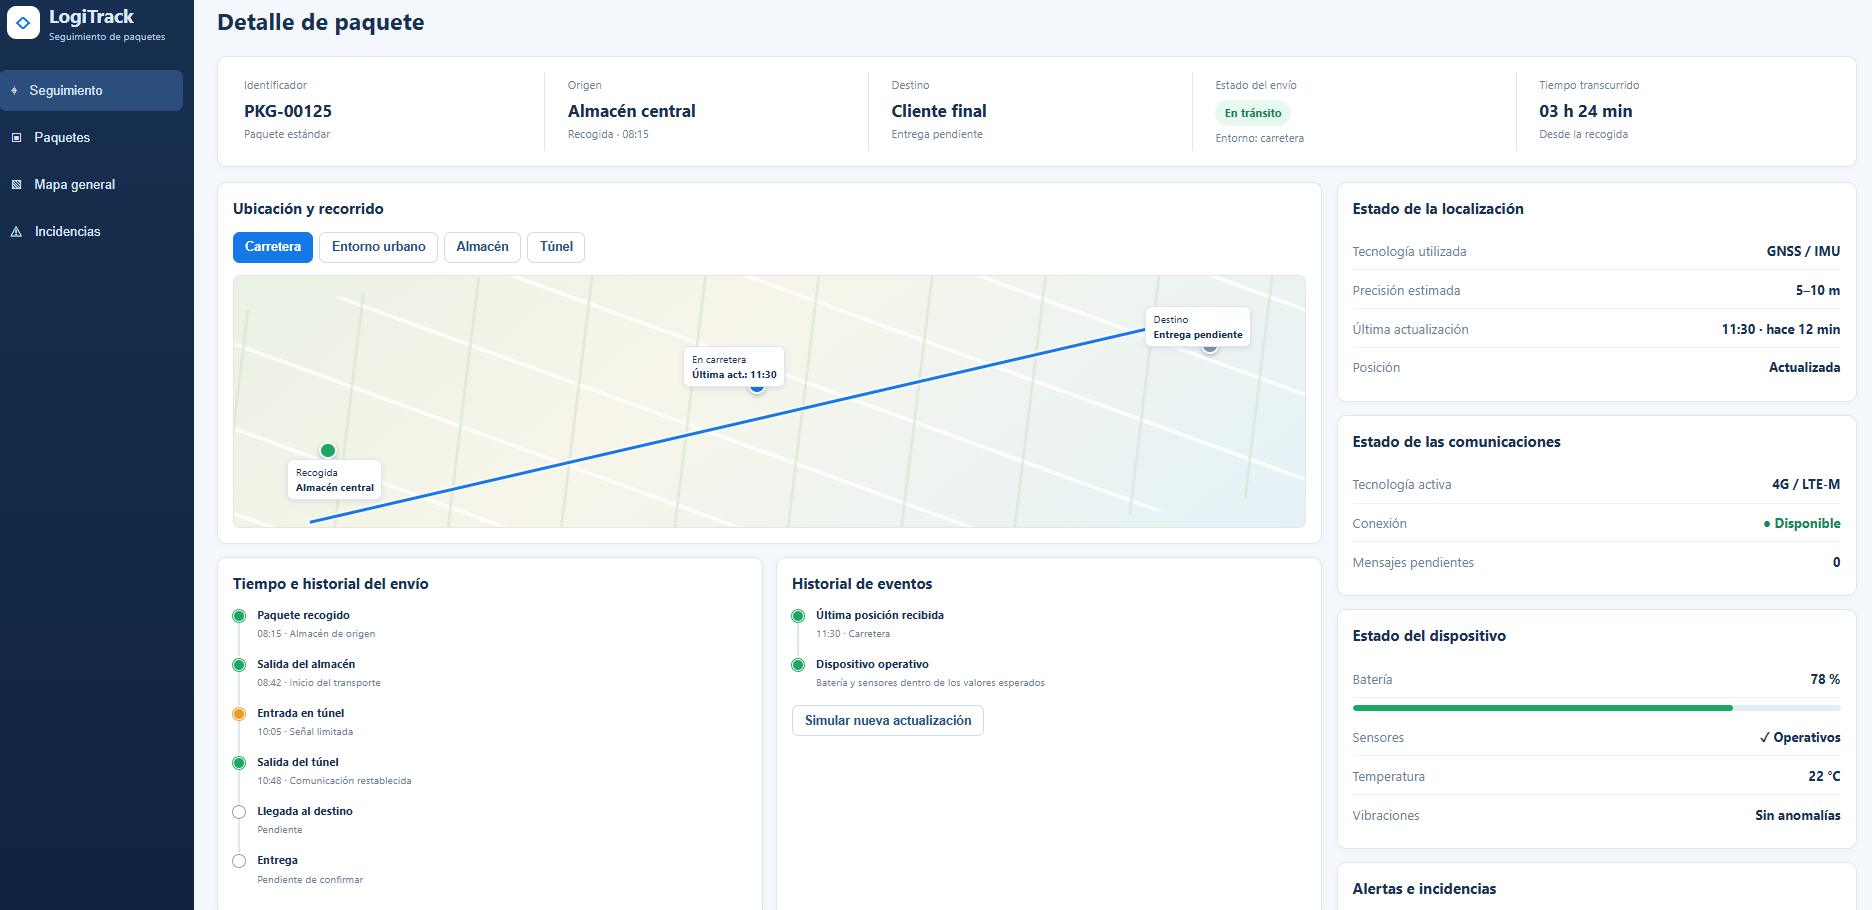
\includegraphics[width=0.85\textwidth]{logitrack_carretera.png}
    \caption{Interfaz de la aplicación de gestión en el entorno de carretera.}
    \label{fig:app_carretera}
\end{figure}

\begin{figure}[H]
    \centering
    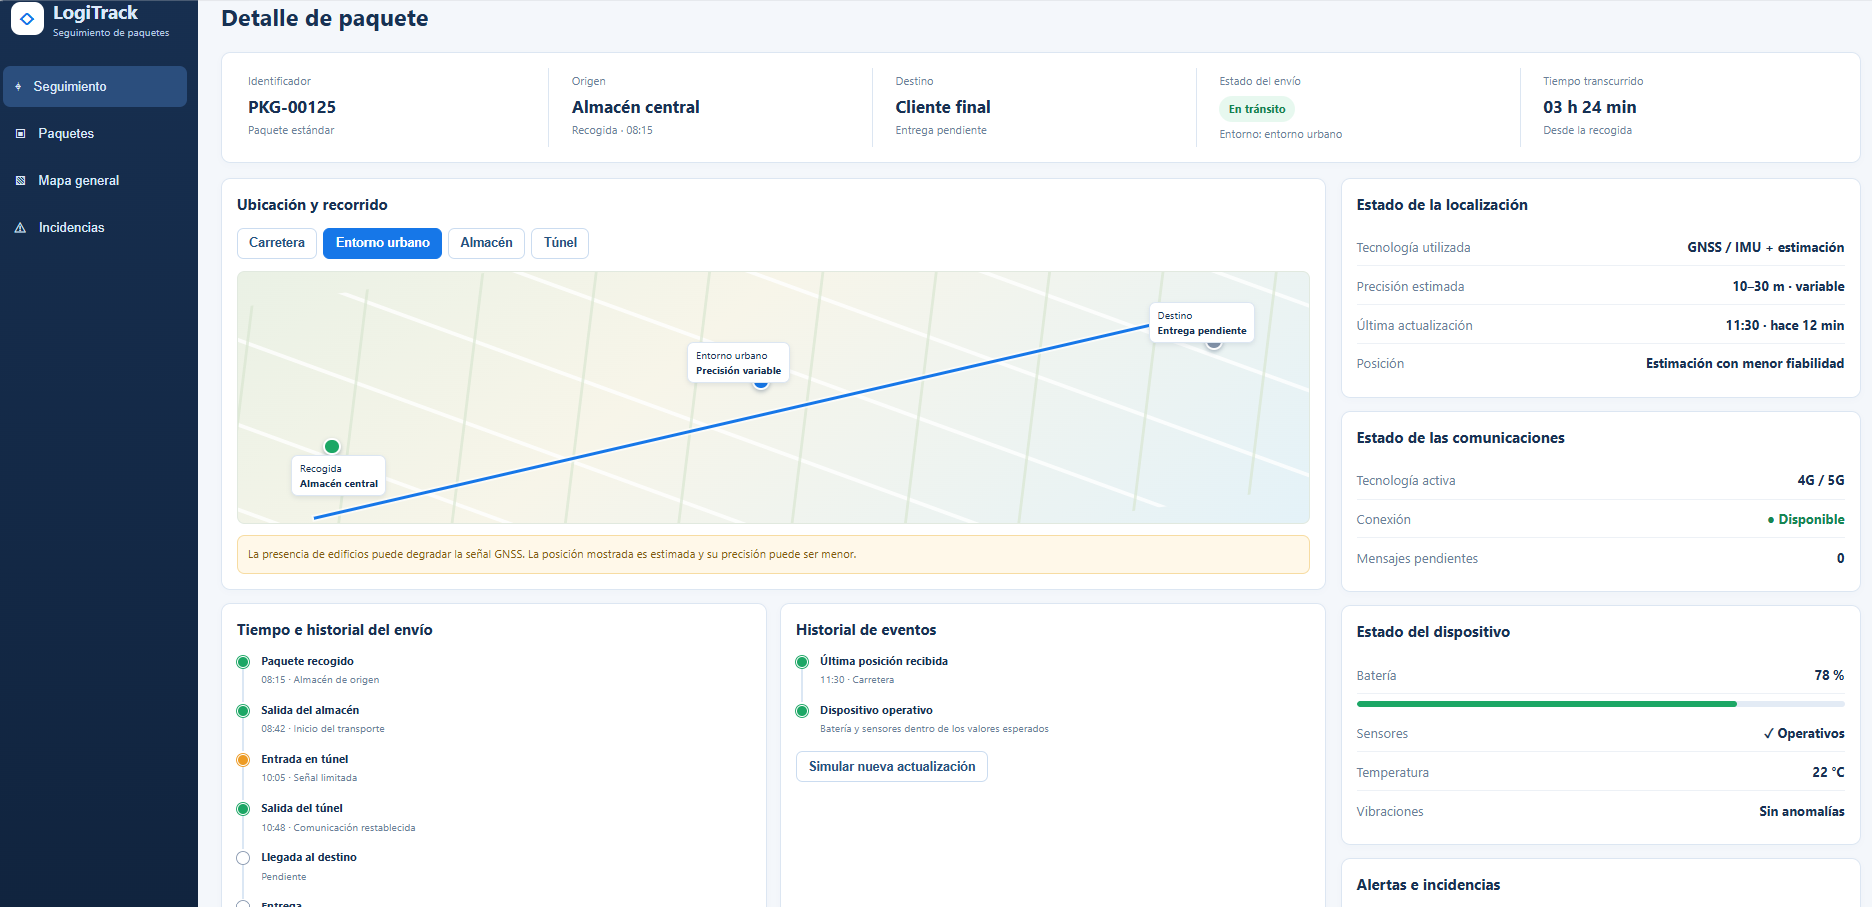
\includegraphics[width=0.85\textwidth]{logitrack_urbano.png}
    \caption{Interfaz de la aplicación de gestión en el entorno urbano.}
    \label{fig:app_urbano}
\end{figure}

\begin{figure}[H]
    \centering
    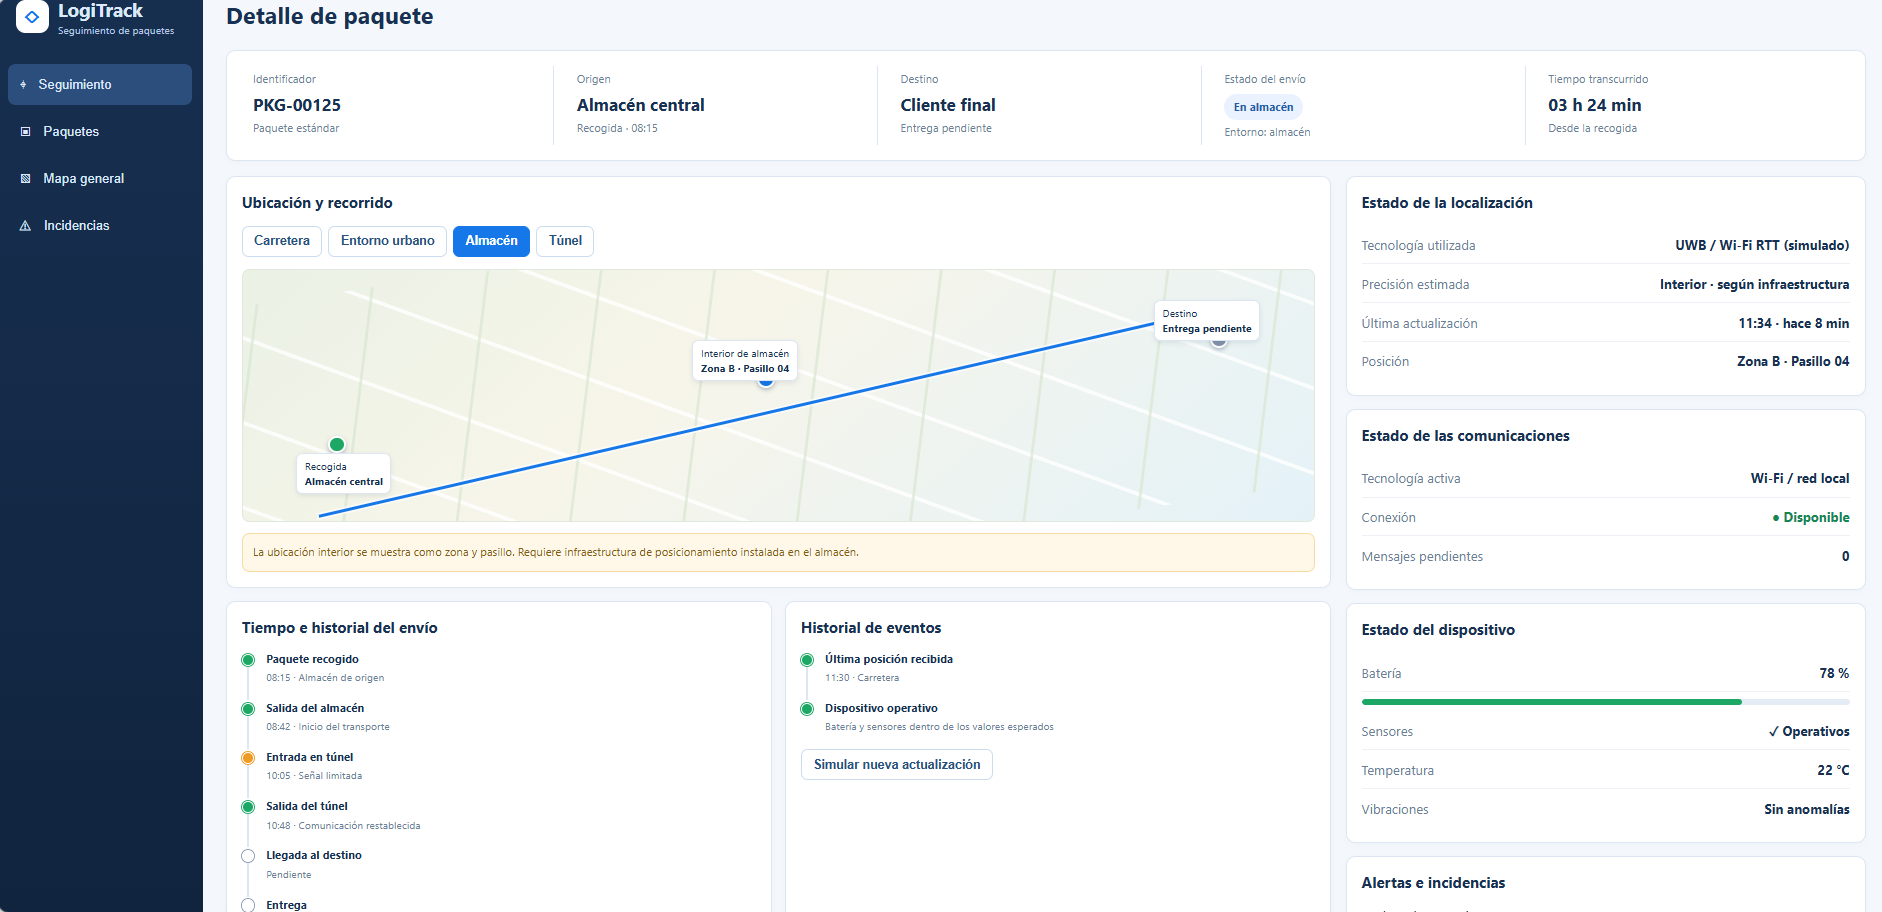
\includegraphics[width=0.85\textwidth]{logitrack_almacen.png}
    \caption{Interfaz de la aplicación de gestión en el entorno de almacén.}
    \label{fig:app_almacen}
\end{figure}

\begin{figure}[H]
    \centering
    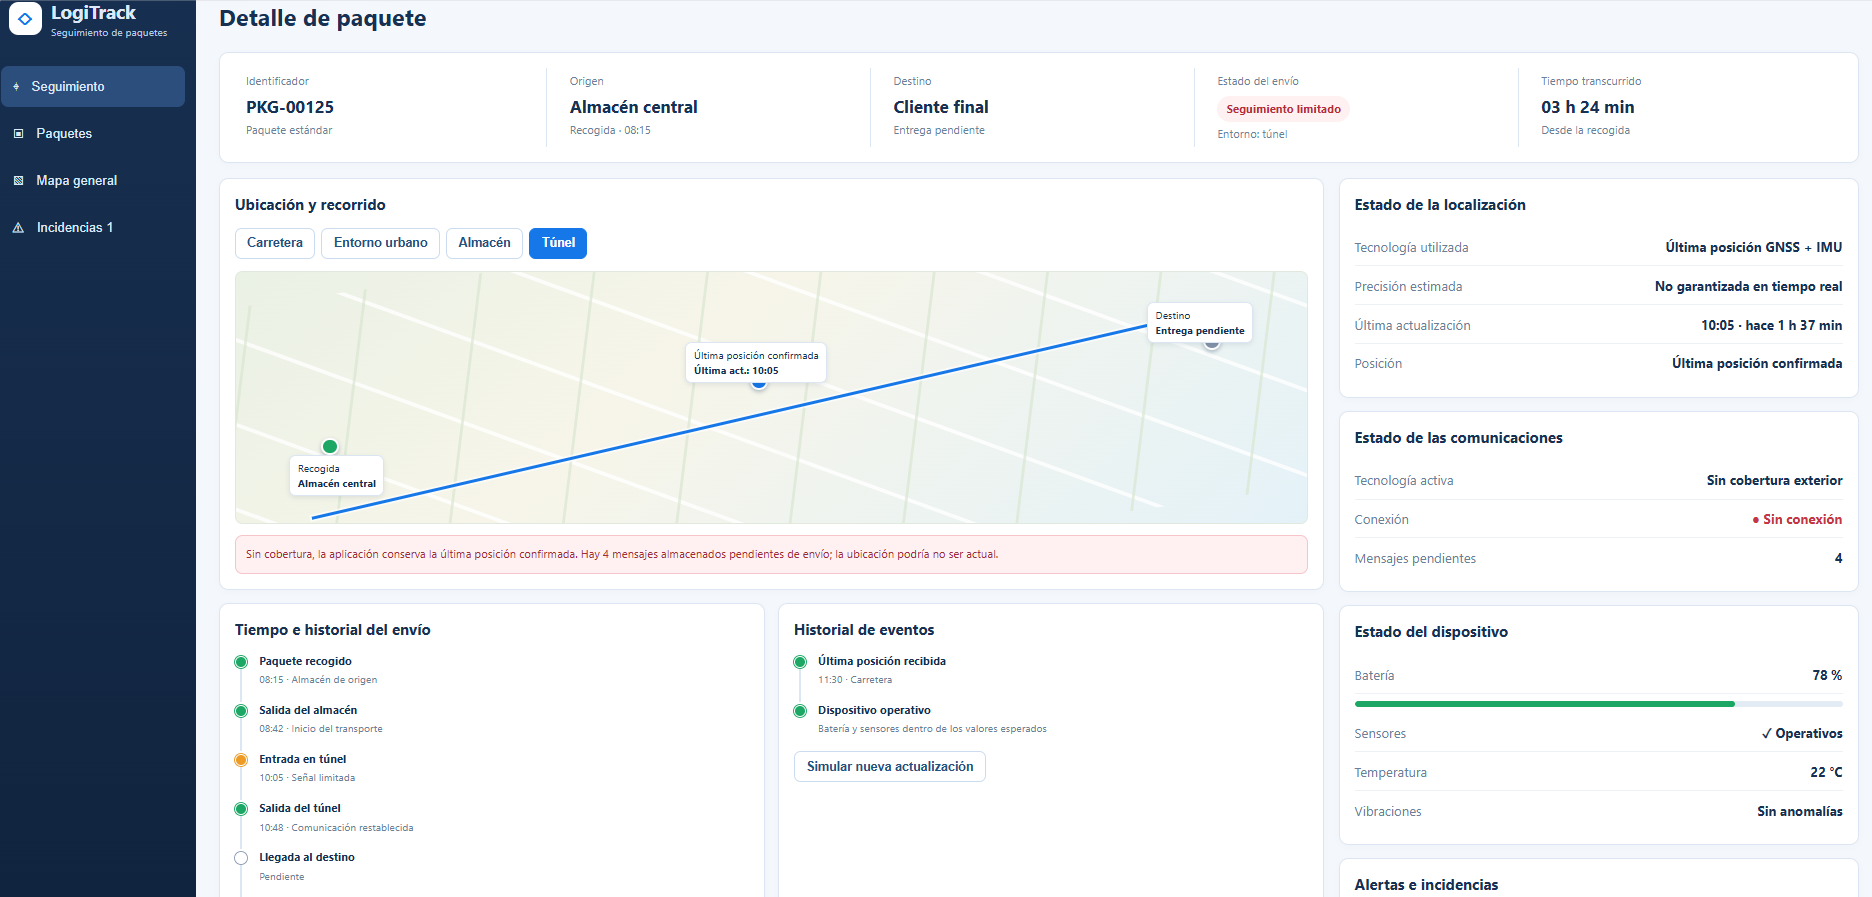
\includegraphics[width=0.85\textwidth]{logitrack_tunel.png}
    \caption{Interfaz de la aplicación de gestión en el entorno de túnel.}
    \label{fig:app_tunel}
\end{figure}

El enlace al repositorio donde se puede bajar el HTML de la app simulada es el siguiente: \url{https://github.com/lusilux/SCO/blob/main/logitrackv2.html}.

% =================================================================
% 9. CONCLUSIONES
% =================================================================
\clearpage
\section{Conclusiones}
\label{sec:apartado9}

En este trabajo se ha propuesto un sistema de seguimiento de paquetes capaz de registrar su ubicación y calcular el tiempo transcurrido desde su recogida hasta su entrega, teniendo en cuenta las condiciones de localización y comunicación que aparecen durante el proceso de transporte.

La propuesta combina tecnologías como GNSS para exteriores y UWB para interiores y túneles, junto con redes móviles y una infraestructura de comunicación específica en zonas sin cobertura. Además, el almacenamiento local y el reenvío de mensajes permiten mantener la trazabilidad de los paquetes ante posibles interrupciones de la conexión.

En definitiva, nuestro estudio muestra que es posible obtener una solución integral combinando tecnologías existentes, siempre que se tengan en cuenta sus limitaciones. Como trabajo futuro, sería necesario validar la propuesta mediante pruebas de campo que permitan comprobar la validez del sistema.

% =================================================================
% BIBLIOGRAFÍA (orden de primera aparición en el texto)
% =================================================================
\newpage
\phantomsection
\addcontentsline{toc}{section}{Bibliografía}
\renewcommand{\refname}{Bibliografía}
\begin{thebibliography}{99}
    \setlength{\itemsep}{2pt}

    \bibitem{ref1} United States. Department of Defense. \emph{Global Positioning System Standard Positioning Service Performance Standard}. \url{https://rosap.ntl.bts.gov/view/dot/16930}

    \bibitem{ref2} National Institute of Standards and Technology (NIST). \emph{Indoor Localization at NIST}. \url{https://www.nist.gov/ctl/pscr/indoor-localization-nist}

    \bibitem{ref3} Jiang, S., Xu, Q., Wang, W., Peng, P., \& Li, J. \emph{Vehicle positioning systems in tunnel environments: a review}. Complex \& Intelligent Systems, 11, 164 (2025). \url{https://doi.org/10.1007/s40747-024-01744-1}

    \bibitem{ref4} Almuhaya, M. A. M., Jabbar, W. A., Sulaiman, N., \& Abdulmalek, S. \emph{A Survey on LoRaWAN Technology: Recent Trends, Opportunities, Simulation Tools and Future Directions}. Electronics, 11, 164 (2022). \url{https://doi.org/10.3390/electronics11010164}

    \bibitem{ref5} Stone, W. C. \emph{Electromagnetic Signal Attenuation in Construction Materials}. National Institute of Standards and Technology (NIST), NISTIR 6055 (1997). \url{https://doi.org/10.6028/NIST.IR.6055}

    \bibitem{ref6} Jaeckel, S., Turay, N., Raschkowski, L., Thiele, L., Vuohtoniemi, R., Sonkki, M., Hovinen, V., Burkhardt, F., Karunakaran, P., \& Heyn, T. \emph{Industrial Indoor Measurements from 2-6 GHz for the 3GPP-NR and QuaDRiGa Channel Model}. IEEE 90th Vehicular Technology Conference (VTC2019-Fall) (2019). \url{https://arxiv.org/abs/1906.12145}

    \bibitem{ref7} IEEE. \emph{Wave Propagation Modeling Techniques in Tunnel Environments: A Survey}. IEEE Journals \& Magazine. \url{https://ieeexplore.ieee.org/document/10005074}

    \bibitem{ref8} GPS.gov. \emph{GPS Accuracy}. \url{https://www.gps.gov/gps-accuracy}

    \bibitem{ref9} Unión Internacional de Telecomunicaciones (ITU-R). \emph{Recomendación ITU-R P.1406-2: Propagation effects relating to terrestrial land mobile and broadcasting services in the VHF and UHF bands}. \url{https://www.itu.int/dms_pubrec/itu-r/rec/p/R-REC-P.1406-2-201507-I!!PDF-E.pdf}

    \bibitem{ref10} European Space Agency (ESA). \emph{Indoor satellite navigation}. \url{https://www.esa.int/Enabling_Support/Space_Engineering_Technology/Indoor_satellite_navigation}

    \bibitem{ref11} Unión Internacional de Telecomunicaciones (ITU-R). \emph{Leaky-feeder systems in the land mobile service} (Report M.902-1, 1990). \url{https://www.itu.int/dms_pub/itu-r/opb/rep/r-rep-m.902-1-1990-pdf-e.pdf}

    \bibitem{ref12} GSMA. \emph{Mobile IoT (LPWA)}. \url{https://www.gsma.com/solutions-and-impact/technologies/internet-of-things/mobile-iot/}

    \bibitem{ref13} LoRa Alliance. \emph{LoRaWAN for Developers}. \url{https://lora-alliance.org/lorawan-for-developers/}

    \bibitem{ref14} Asante e Imamura (2026). \emph{Seamless Indoor and Outdoor Navigation Using IMU-GNSS Sensor Data Fusion}. \url{https://pmc.ncbi.nlm.nih.gov/articles/PMC13075324/}

    \bibitem{ref15} Amazon Web Services. \emph{Implementing Low-Power Wide-Area Network (LPWAN) Solutions with AWS IoT: LTE-M}. \url{https://docs.aws.amazon.com/whitepapers/latest/implementing-lpwan-solutions-with-aws/lte-m.html}

    \bibitem{ref16} Ng et al. (2021). \emph{Urban positioning: 3D mapping-aided GNSS using dual-frequency pseudorange measurements from smartphones}. \url{https://doi.org/10.1002/navi.448}

    \bibitem{ref17} National Institute of Standards and Technology (NIST). \emph{Ultra-Wideband Location}. \url{https://www.nist.gov/ctl/wireless-networks-division/ultra-wideband-location}

    \bibitem{ref18} Android Developers. \emph{Wi-Fi location: ranging with RTT}. \url{https://developer.android.com/develop/connectivity/wifi/wifi-rtt}

    \bibitem{ref19} Bluetooth SIG. \emph{Bluetooth Channel Sounding: How it works and what it means}. \url{https://www.bluetooth.com/blog/bluetooth-channel-sounding-how-it-works/}

    \bibitem{ref20} Jacksha y Sunderman (2018). \emph{Data transport over leaky feeder systems using Internet-Protocol-enabled land mobile radios}. \url{https://pmc.ncbi.nlm.nih.gov/articles/PMC6400079/}

    \bibitem{ref21} Theissen et al. (2025). \emph{LoRa Propagation and Coverage Measurements in Underground Potash Salt Room-and-Pillar Mines}. \url{https://pmc.ncbi.nlm.nih.gov/articles/PMC12197270/}

    \bibitem{ref22} FHNW. \emph{Measurement of 868MHz LoRa radio propagation in a tunnel}. \url{https://irf.fhnw.ch/entities/publication/266c05f2-470b-4a59-9993-f7f34fca245d}

    \bibitem{ref23} Wang et al. (2023). \emph{Research on IMU-Assisted UWB-Based Positioning Algorithm in Underground Coal Mines}. \url{https://pmc.ncbi.nlm.nih.gov/articles/PMC10384321/}

    \bibitem{ref24} The Things Network. \emph{LoRaWAN Architecture}. \url{https://www.thethingsnetwork.org/docs/lorawan/architecture/}

    \bibitem{ref25} IEEE Std 802.15.4z-2020. \emph{IEEE Standard for Low-Rate Wireless Networks---Amendment 1: Enhanced Ultra Wideband (UWB) Physical Layers (PHYs) and Associated Ranging Techniques}. \url{https://standards.ieee.org/ieee/802.15.4z/10230/}

    \bibitem{ref26} LoRa Alliance. \emph{RP002-1.0.4 LoRaWAN Regional Parameters} (ciclo de trabajo en EU868). \url{https://resources.lora-alliance.org/document/rp002-1-0-4-regional-parameters}

    \bibitem{ref27} The Things Network. \emph{Regional Limitations of RF Use} (límites de ciclo de trabajo por subbanda). \url{https://www.thethingsnetwork.org/docs/lorawan/regional-limitations-of-rf-use/}

    \bibitem{ref28} ETSI EN 300 220-2 V3.2.1 (2018). \emph{Short Range Devices (SRD) operating in the frequency range 25 MHz to 1 000 MHz; Part 2: Harmonised Standard for access to radio spectrum for non specific radio equipment}. \url{https://www.etsi.org/deliver/etsi_en/300200_300299/30022002/03.02.01_60/en_30022002v030201p.pdf}

    \bibitem{ref29} Shelby et al. (2014). \emph{RFC 7252, The Constrained Application Protocol (CoAP)}. \url{https://www.rfc-editor.org/rfc/rfc7252}

    \bibitem{ref30} OASIS (2019). \emph{MQTT Version 5.0}. \url{https://docs.oasis-open.org/mqtt/mqtt/v5.0/mqtt-v5.0.html}

    \bibitem{ref31} Vliegen (2026). \emph{Tracking Mobile Assets in GPS Deprived Environments} (CERN Bachelor Thesis Defense). \url{https://prezi.com/page/x9iumsaq_vgx/tracking-mobile-assets-in-gps-deprived-environments}

    \bibitem{ref32} Wikipedia. \emph{Leaky feeder}. \url{https://en.wikipedia.org/wiki/Leaky_feeder}

    \bibitem{ref33} Udugampola et al. (2025). \emph{A Position- and Energy-Aware Routing Strategy for Subterranean LoRa Mesh Networks} (arXiv). \url{https://arxiv.org/html/2510.03714v1}

    \bibitem{ref34} Shanmuga Sundaram, Du y Zhao (2019). \emph{A Survey on LoRa Networking: Research Problems, Current Solutions and Open Issues} (arXiv). \url{https://arxiv.org/pdf/1908.10195}

    \bibitem{ref35} LoRa Alliance (2020). \emph{TS001-1.0.4 LoRaWAN L2 1.0.4 Specification}. \url{https://resources.lora-alliance.org/home/ts001-1-0-4-lorawan-l2-1-0-4-specification}

    \bibitem{ref36} Lansitec. \emph{Tracking Label} (ThingsBoard IoT Hub). \url{https://thingsboard.io/iot-hub/devices/tracking-label/}

    \bibitem{ref37} Lansitec. \emph{Asset Management Tracker} (ThingsBoard IoT Hub). \url{https://thingsboard.io/device-library/asset-management-tracker/}

    \bibitem{ref38} Cerf et al. (2007). \emph{RFC 4838, Delay-Tolerant Networking Architecture}. \url{https://www.rfc-editor.org/rfc/rfc4838}

    \bibitem{ref39} IEEE Std 802.3at-2009. \emph{Data Terminal Equipment (DTE) Power via the Media Dependent Interface (MDI) Enhancements (Power over Ethernet Plus)}. \url{https://standards.ieee.org/products-services/standards/ieee-802-3at}

    \bibitem{ref40} ETSI EN 302 065-1 V2.1.1 (2016). \emph{Short Range Devices (SRD) using Ultra Wide Band technology (UWB); Part 1: Requirements for Generic UWB applications}. \url{https://www.etsi.org/deliver/etsi_en/302000_302099/30206501/02.01.01_60/en_30206501v020101p.pdf}

    \bibitem{ref41} ECC Recommendation (10)02 (2010). \emph{A framework for authorisation regime of Global Navigation Satellite System (GNSS) repeaters}. \url{https://docdb.cept.org/document/495}

    \bibitem{ref42} oneM2M. \emph{An Introduction to oneM2M's Architecture}. \url{https://recipes.onem2m.org/introduction/Introduction-to-oneM2M-Architecture}

    \bibitem{ref43} The Things Industries. \emph{Application Server} (The Things Stack Documentation). \url{https://www.thethingsindustries.com/docs/concepts/architecture/components/application-server/}

    \bibitem{ref44} ThingsBoard. \emph{Rule Engine} (Documentation). \url{https://thingsboard.io/docs/user-guide/rule-engine/}

    \bibitem{ref45} Reglamento (UE) 2016/679 del Parlamento Europeo y del Consejo, de 27 de abril de 2016 (RGPD), texto consolidado en BOE. \url{https://www.boe.es/buscar/doc.php?id=DOUE-L-2016-80807}

    \bibitem{ref46} IETF (2011). \emph{RFC 6455, The WebSocket Protocol}. \url{https://www.rfc-editor.org/rfc/rfc6455.html}

    \bibitem{ref47} The Things Industries. \emph{Webhooks} (The Things Stack Documentation). \url{https://www.thethingsindustries.com/docs/integrations/webhooks/retries}

    \bibitem{ref48} OWASP. \emph{API Security Top 10, edición 2023}. \url{https://owasp.org/API-Security/editions/2023/en/0x11-t10/}

    \bibitem{ref49} NIST (2020). \emph{NISTIR 8259A, IoT Device Cybersecurity Capability Core Baseline}. \url{https://nvlpubs.nist.gov/nistpubs/ir/2020/NIST.IR.8259A.pdf}
\end{thebibliography}

\end{document}
